

\PassOptionsToPackage{table}{xcolor} % to use colors in tables
\PassOptionsToPackage{pdfa}{hyperref}
\documentclass{unipd-thesis-modern} % src: https://github.com/baronefr/unipd-


% additional packages
\usepackage{lipsum} % for DEMO only
\usepackage{threeparttable}
\usepackage{threeparttable}
\usepackage{siunitx}
\usepackage[titles]{tocloft} % to modify spacing in toc chapters
\usepackage{tabularx}
\usepackage{booktabs}
\usepackage{caption}
\usepackage{array}
\usepackage[utf8]{inputenc}
\usepackage{titlesec} % Paquete para controlar espaciado de títulos
\usepackage{graphicx}
\usepackage{float} % para usar [H] si quieres fijar la figura
\usepackage{geometry}
\usepackage{pdflscape}
\usepackage{tabularx}
\usepackage{booktabs}
\usepackage{threeparttable}
\usepackage{listings}
\renewcommand{\tabularxcolumn}[1]{m{#1}}
\usepackage{longtable}

\definecolor{codebg}{RGB}{248,249,251}
\definecolor{codeframe}{RGB}{210,214,220}
\definecolor{codekw}{RGB}{17,87,158}
\definecolor{codecom}{RGB}{93,109,126}
\definecolor{codestr}{RGB}{135,54,0}
\definecolor{codenum}{RGB}{120,120,120}

\lstdefinestyle{thesiscode}{
    basicstyle=\ttfamily\footnotesize,
    frame=single,
    framerule=0.4pt,
    rulecolor=\color{codeframe},
    backgroundcolor=\color{codebg},
    breaklines=true,
    breakatwhitespace=false,
    columns=fullflexible,
    keepspaces=true,
    showstringspaces=false,
    upquote=true,
    numbers=left,
    numberstyle=\scriptsize\color{codenum},
    numbersep=6pt,
    keywordstyle=\bfseries\color{codekw},
    commentstyle=\itshape\color{codecom},
    stringstyle=\color{codestr},
    tabsize=2,
    xleftmargin=0.6em,
    xrightmargin=0.2em,
    framexleftmargin=0.5em,
    aboveskip=0.7em,
    belowskip=0.7em,
    captionpos=b,
    abovecaptionskip=0.4em,
    belowcaptionskip=0.2em
}

\usepackage{listings}
\usepackage{xcolor}

\lstdefinestyle{code}{
    basicstyle=\ttfamily\small,
    keywordstyle=\color{blue},
    commentstyle=\color{gray},
    stringstyle=\color{green!50!black},
    numbers=left,
    numberstyle=\tiny,
    breaklines=true,
    frame=single
}



\setlength{\cftbeforechapskip}{7pt}
\setcounter{tocdepth}{4} % ToC depth


% titles
\title{Metodología Basada en Métodos de Ciencia de Datos para Predecir los Indicadores de Calidad del Servicio (SAIDI y SAIFI) en Redes de Distribución de una Empresa de Energía Eléctrica en el Norte de Santander}
\thesisHeader{Pontificia Universidad Javeriana Cali \\Facultad de Ingeniería y Ciencias.\\MAESTRÍA EN CIENCIA DE DATOS}
\academicYear{07-2024/11-2024}

% student
\author{Edwin Henao Ochoa\\
Cindy Lugo Rozo\\
Edwin Silva Salas}

% supervisor(s)Zürich
\advisor{Sandra Milena Ramírez Buelvas}{Pontificia Universidad Javeriana} % (mandatory)
%\coadvisor{xxxxx }{xxxxx} 
% (optional, comment to remove)
%\otheradvisor{Prof. Paolino Paperino}{University of Padua} % (optional, comment to remove)
% ^ NOTE: you can use optional arg to customize the label "Internal Supervisor"
%   example:   \otheradvisor[The best supervisor!]{Prof. Paolino Paperino}{University of Padua}

% dedication (comment to remove)
\dedication{\textit{A nuestras familias y amigos \\ Edwin Henao Ochoa\\
Cindy Lugo Rozo\\
Edwin Silva Salas}}

% custom symbols (optional)
\input{custom-symbols}

% bibliography file
\addbibresource{refs.bib}

\sisetup{
  output-decimal-marker = {.},
  group-separator = {,},
  detect-all = true
}


% Ajustes de espacio
\titlespacing*{\subsection}{0pt}{10pt plus 2pt minus 2pt}{5pt}
\titlespacing*{\subsubsection}{0pt}{5pt plus 2pt minus 2pt}{3pt}
% Otros paquetes y configuraciones
\setlength{\intextsep}{6pt}      % Espacio entre texto y figuras
\setlength{\textfloatsep}{6pt}   % Espacio entre texto y flotantes


\begin{document}
\renewcommand{\tablename}{Tabla}
\renewcommand{\listfigurename}{Lista de figuras}
\renewcommand{\listtablename}{Lista de tablas}
    \frontmatter
    % --------------------------
    
\chapter*{Introducción}
\addcontentsline{toc}{chapter}{Introducción}

Sin duda, la energía eléctrica es vital para el progreso de cada región, tanto social, económica como industrialmente. En Colombia, el acceso a este servicio está estrictamente regulado en términos de provisión, con el objetivo de asegurar que todos los usuarios cuenten con un suministro de energía constante, seguro y de alta calidad para vivir y trabajar~\cite{ref1}. Los operadores de red tienen de manera continua la responsabilidad de garantizar que la entrega de energía sea confiable para hogares, instituciones y negocios, evitando fallas en la prestación del servicio en cualquier tipo de edificación.

No obstante, esta tarea no es sencilla. La operación de los sistemas de distribución de energía se ve afectada por múltiples factores técnicos, ambientales y operativos, así como por la duración y frecuencia de las interrupciones del servicio. En este contexto, la Comisión de Regulación de Energía y Gas (CREG) adoptó los indicadores SAIDI (Índice de Duración Promedio de Interrupción del Sistema) y SAIFI (Índice de Frecuencia Promedio de Interrupción del Sistema) como los criterios oficiales para evaluar la calidad del servicio en las redes de distribución, mediante la Resolución CREG 015 de 2018 \cite{ref1}. Estos indicadores permiten evaluar el desempeño operativo y facilitan la implementación de esquemas de compensación y control por parte de la Superintendencia de Servicios Públicos Domiciliarios (SSPD) \cite{ref4}.

Sin embargo, la gestión efectiva de estos indicadores ha resultado compleja, dada la heterogeneidad de los eventos que originan las interrupciones y la limitada conectividad de la información almacenada en sistemas dispares como SCADA, OMS, GIS, CIS y bases de datos externas.\footnote{SCADA (\textit{Supervisory Control and Data Acquisition}): sistema de supervisión y adquisición de datos de la operación de la red. OMS (\textit{Outage Management System}): sistema de gestión de interrupciones. GIS (\textit{Geographic Information System}): sistema de información geográfica de activos. CIS (\textit{Customer Information System}): sistema de información de clientes.} Debido a que los registros operativos, climáticos y de mantenimiento se encuentran dispersos y fragmentados en múltiples plataformas, construir modelos analíticos capaces de pronosticar la frecuencia y el tiempo de duración de interrupciones eléctricas en distintas áreas o circuitos representa un desafío significativo.

Esta brecha limita la capacidad de las empresas para tomar decisiones oportunas, priorizar inversiones, mejorar la planificación del mantenimiento y responder adecuadamente a los requerimientos regulatorios. En consecuencia, resulta fundamental desarrollar herramientas apoyadas en ciencia de datos que permitan consolidar información histórica, identificar patrones relevantes y pronosticar la frecuencia y el tiempo de duración de interrupciones eléctricas.

Este trabajo presenta técnicas para la recopilación de datos provenientes de plataformas operativas internas y fuentes externas, así como el análisis de modelos estadísticos y de aprendizaje automático orientados al \textbf{pronóstico de la frecuencia y el tiempo de duración de interrupciones eléctricas} en una empresa de distribución de energía que opera en el departamento de Norte de Santander, en el marco de los indicadores regulatorios SAIDI y SAIFI. Al adoptar esta estrategia, se busca anticipar cuándo y con qué intensidad operativa pueden ocurrir las interrupciones, e identificar las influencias técnicas, operativas y climáticas más relevantes en la continuidad del servicio. Este desarrollo constituye una contribución significativa para fortalecer la toma de decisiones basada en evidencia, optimizar los planes de mantenimiento, apoyar el cumplimiento regulatorio y ofrecer un caso académico aplicado sobre el uso de técnicas analíticas en el sector eléctrico regulado, beneficiando a más de 600{.}000 usuarios.

El documento se organiza de la siguiente manera. En la Sección~\ref{sec:problema} se presenta el planteamiento y la formulación del problema de continuidad del servicio. En la Sección~\ref{sec:objetivos} se exponen el objetivo general y los objetivos específicos, alineados con las preguntas de investigación. En la Sección~\ref{sec:marco-referencia} se desarrolla el marco teórico (definiciones regulatorias de SAIDI y SAIFI, exclusiones y factores asociados) y los antecedentes sobre modelación de interrupciones e indicadores de confiabilidad. En la Sección~\ref{sec:datos} se describe la fuente y la estructura de los datos empleados. En la Sección~\ref{sec:metodologia} se detallan las etapas metodológicas ---desde la extracción e integración hasta el EDA, la ingeniería de variables y el modelamiento--- orientadas al pronóstico de la frecuencia y el tiempo de duración de interrupciones eléctricas. Posteriormente, en la Sección~\ref{sec:resultados} se presentan los resultados por etapa; en la Sección~\ref{sec:discusion} se discute el alcance, los aportes y las limitaciones frente a cada objetivo; y en la Sección~\ref{sec:conclusion} se consolidan las conclusiones del trabajo.

    \newpage
    % --------------------------
    \mainmatter
    % --------------------------
    \chapter{Definición del problema}
    
\section{Planteamiento del problema}

\subsection{Planteamiento del problema}

Los indicadores de continuidad del servicio SAIDI (Índice de Duración Promedio de Interrupción del Sistema) y SAIFI (Índice de Frecuencia Promedio de Interrupción del Sistema) en la empresa de distribución objeto de estudio presentan dificultades estructurales para su mejora sostenida. Si bien existen técnicas estadísticas y de aprendizaje automático ampliamente documentadas para el análisis de interrupciones en sistemas eléctricos, la principal limitación no radica en la ausencia de metodologías analíticas, sino en la calidad, estructura e interpretación de los datos disponibles, lo que dificulta el entrenamiento de modelos predictivos que sean simultáneamente confiables y explicativos \cite{ref1,ref4,ref3}. En particular, resulta complejo detectar, cuantificar y explicar no solo las causas de las interrupciones, sino también su duración y los tiempos de restauración del servicio.

Los principales obstáculos identificados son los siguientes:

\begin{itemize}
    \item \textbf{Fragmentación de las fuentes de información}: La operación del sistema requiere el uso de múltiples registros provenientes de plataformas heterogéneas como SCADA, OMS, GIS, CIS, bases de mantenimiento y fuentes meteorológicas externas. Estos datos se encuentran en distintos formatos, con estructuras disímiles y, en algunos casos, con ausencia de metadatos completos, lo que dificulta su integración sin pérdida de trazabilidad \cite{ref5,ref6}.
    \item \textbf{Problemas de sincronización temporal}: Los sistemas operativos no presentan una alineación temporal uniforme. Mientras algunos registran información en intervalos horarios, otros lo hacen en escalas de minutos o presentan series discontinuas. Esta falta de sincronización genera inconsistencias que afectan la estimación precisa de la duración de las interrupciones y de los tiempos de reposición del servicio \cite{ref5,ref7}.
    \item \textbf{Eventos extremos y ruido en los datos}: Los registros contienen alta variabilidad, errores de captura, información incompleta y eventos atípicos, como fenómenos climáticos extremos o fallas excepcionales, que suelen ser excluidos del análisis. Esta situación dificulta la identificación de patrones robustos tanto a nivel agregado como local \cite{ref1,ref8}.
    \item \textbf{Pérdida de detalle por agregación}: El uso de indicadores promediados en escalas anuales o geográficas amplias oculta el comportamiento específico de circuitos o zonas particulares, lo que limita la identificación de causas operativamente accionables \cite{ref4,ref7}.
    \item \textbf{Ausencia de estándares de datos}: La falta de catálogos de datos, definiciones homogéneas y métricas de integridad impide evaluar de manera sistemática si las fuentes disponibles son adecuadas para la construcción de modelos predictivos confiables \cite{ref5,ref6}.
    \item \textbf{Restricciones regulatorias}: Los organismos de control exigen que los resultados sean trazables y explicables. En consecuencia, no es suficiente emplear modelos con alto desempeño predictivo; estos deben ser interpretables y compatibles con los requerimientos de reporte regulatorio, lo que condiciona el tipo de metodologías que pueden adoptarse \cite{ref3,ref4}.
\end{itemize}

Estos obstáculos reducen la capacidad de la organización para explicar la variación de los indicadores SAIDI y SAIFI, priorizar actividades operativas y cumplir con los requerimientos regulatorios mediante herramientas predictivas \cite{ref3,ref8,ref5}. En términos cuantitativos, el SAIDI promedio de la empresa es de 22.43 horas por año, valor que se ubica un 4.64\% por debajo de la meta establecida por la CREG (23.522 horas por año). Para el indicador SAIFI, el promedio anual es de 6.5 eventos, significativamente inferior al objetivo regulatorio de 9 eventos por año, lo que representa una reducción del 27.78\% \cite{ref43}. Estos resultados sugieren que la empresa se encuentra dentro de los límites regulatorios; sin embargo, la gestión de dichos indicadores enfrenta importantes desafíos operativos e informativos.

Las compensaciones anuales asociadas a calidad del servicio ascienden aproximadamente a \$5 mil millones de pesos, y el análisis de datos históricos de cinco años evidencia que cerca del 2\% de los registros presenta información faltante o inconsistente, como tiempos de evento no registrados, campos incompletos o desajustes temporales entre sistemas. Si bien la Circular 063 de 2019 de la SSPD establece criterios técnicos para la exclusión válida de eventos asociados a factores externos, como fuerza mayor o fallas del Sistema Nacional de Transmisión, la presencia de problemas de calidad de datos limita la capacidad de construir modelos predictivos sólidos, diagnosticar con precisión las causas de las interrupciones y priorizar acciones operativas basadas en evidencia \cite{ref1,ref4,ref3,ref44}.

Este problema no es exclusivo de la empresa analizada. En el sector eléctrico colombiano, la calidad del servicio constituye un desafío estructural. De acuerdo con el Informe de Calidad del Servicio de Energía Eléctrica de la SSPD 2023, el SAIDI promedio nacional fue de 16.83 horas por usuario, con valores que oscilaron entre 4.5 horas y más de 50 horas dependiendo del operador y de la región geográfica \cite{ref9}. Esta dispersión refleja diferencias significativas en infraestructura, gestión operativa y exposición a condiciones climáticas extremas. Durante 2023, el 68\% de las interrupciones estuvo asociado a eventos externos, como contacto con vegetación, animales o terceros, mientras que el 24\% se atribuyó a fallas técnicas en equipos de red, evidenciando la naturaleza multicausal del problema \cite{ref4}.

El impacto regulatorio es considerable: en 2023, las compensaciones totales por incumplimiento de metas de calidad alcanzaron aproximadamente \$487\,000 millones a nivel nacional, siendo los indicadores de continuidad responsables del 73\% de este valor \cite{ref4}. Para operadores de red ubicados en zonas con alta exposición climática, como Norte de Santander, la problemática se intensifica. Según datos de la SSPD consolidados por la UPME, los eventos meteorológicos extremos incrementaron en un 35\% las interrupciones no programadas respecto al periodo 2019--2021 \cite{ref4}. En este contexto, la dispersión de información en sistemas heterogéneos dificulta la identificación de patrones causales, la priorización del mantenimiento preventivo y la detección temprana de circuitos críticos, limitando la capacidad de las empresas distribuidoras para anticipar deterioros en la continuidad del servicio y cumplir de manera consistente con los objetivos regulatorios establecidos por la CREG.

    \newpage
    \section{Formulación del problema}


¿Cómo desarrollar una metodología basada en métodos de ciencia de datos  para pronosticar la frecuencia y el tiempo de duración de interrupciones eléctricas (SAIDI y SAIFI) a nivel de zonas en redes de distribución de una empresa de energía eléctria, ubicada en Norte de Santander, identificando los factores que más influyen en su comportamiento.?

A partir de la formulación anterior, se derivan las siguientes preguntas de sistematización:

\begin{enumerate}
    \item ¿Cómo consolidar un repositorio analítico unificado y trazable que integre SCADA, OMS, GIS, CIS, registros de mantenimiento y datos climáticos, acompañado de un catálogo de datos y métricas de calidad que permitan para pronosticar la frecuencia y el tiempo de duración de interrupciones eléctricas?
    
    \item ¿Qué patrones temporales, espaciales, estacionales o comportamientos atípicos caracterizan la variabilidad de SAIDI y SAIFI a nivel de circuito, y de qué manera estos patrones influyen en la comprensión del fenómeno de continuidad del servicio elétrico y en la identificación de los factores que explican sus fluctuaciones?
    
    \item ¿Qué modelos tienen mejor desempeño para pronosticar la frecuencia y el tiempo de duración de interrupciones eléctricas (SAIDI y SAIFI) a nivel de circuito o zona?
    
    \item ¿Cómo construir artefactos reproducibles (notebooks, contenedores, documentación) y reportes técnicos alineados con los entregables del proyecto que faciliten la interpretación operativa y el uso de resultados en priorización de mantenimiento y reportes regulatorios?
\end{enumerate}



    % --------------------------
    \chapter{Objetivos del proyecto} % 
    
\label{sec:objetivos}

\section{Objetivo general}

Desarrollar una metodología basada en métodos de ciencia de datos para predecir los indicadores de calidad del servicio (SAIDI y SAIFI) en redes de distribución de una empresa de energía eléctrica ubicada en Norte de Santander, identificando los factores que más influyen en su comportamiento.
    \section{Objetivos específicos}

\begin{enumerate}
    \item Consolidar las fuentes de datos relevantes (SCADA/OMS, GIS, registros de fallas y mantenimientos, inventarios/SAC y datos climáticos), documentando su cobertura, calidad y limitaciones mediante un catálogo de datos y métricas de integridad.
    
    \item Determinar qué variables operativas, técnicas y climáticas tienen mayor relevancia para predecir la duración y frecuencia de interrupciones (SAIDI y SAIFI) en la zona de estudio a partir de modelos estadísticos o de Machine Learning.
    
    \item Evaluar el desempeño de diferentes métodos estadísticos o de Machine Learning para predecir SAIDI y SAIFI por circuito o zona, considerando la naturaleza de los datos y la interpretabilidad requerida por los gestores.
\end{enumerate}

    % --------------------------
    \chapter{Marco de referencia}
    \label{sec:marco-referencia}


\section{Marco teórico}
\label{sec:Marco-teorico}


\subsection{Contexto del estudio}
    Cuando hablamos de calidad del servicio eléctrico, nos referimos básicamente a entregar energía de forma segura y eficiente, cumpliendo con estándares regulatorios que garanticen continuidad, confiabilidad y estabilidad para todos los tipos de usuarios: residenciales, industriales, comerciales e institucionales. En Colombia, este servicio es esencial y por eso está regulado por la Comisión de Regulación de Energía y Gas (CREG) \cite{ref3}, que ha establecido métricas y estándares específicos para hacer seguimiento a cómo se presta el servicio. Entre estas métricas, dos son particularmente importantes: el SAIDI (\textit{System Average Interruption Duration Index}) y el SAIFI (\textit{System Average Interruption Frequency Index}).

     \begin{enumerate}
          \item \textbf{Definición del SAIDI según la Resolución CREG 015 de 2018:}
           La Resolución CREG 015 de 2018 define el SAIDI como se indica a continuación. En dicha normativa, el \textbf{OR} es el \textbf{Operador de Red} y el \textbf{SDL} es el \textbf{Sistema de Distribución Local}.
            %\ref{eq:saidi_creg_015_2018}
            \begin{quote}
                La calidad media anual del OR se mide a través de los indicadores de duración y frecuencia de los eventos sucedidos en los SDL, que se establecen como se describe a continuación. El indicador SAIDI representa la duración total en horas de los eventos que en promedio percibe cada usuario del SDL de un OR, hayan sido o no afectados por un evento, en un período anual. Se establece mediante la siguiente expresión:     
                \begin{equation}
                    \begin{aligned}
                    SAIDI_{j,t} 
                    &= \dfrac{\sum_{m=1}^{12} \sum_{i=1}^{n} D_{i,u,m} \times NU_{i,u,m}}{UT_{j,m} \times 60},
                    \end{aligned}
                \label{eq:saidi_creg_015_2018}
                \end{equation}
                donde:
                \begin{itemize} 
                    \item $SAIDI_{j,t}$: Indicador de duración promedio por usuario, de los eventos sucedidos en el SDL del OR $j$, durante el año $t$, medido en horas al año. 
                    \item $D_{i,u,m}$: Duración en minutos del evento $i$, sucedido durante el mes $m$, que afectó al activo $u$ perteneciente al SDL del OR $j$. 
                    \item $NU_{i,u,m}$: Número de usuarios que fueron afectados por el evento $i$ sucedido durante el mes $m$, conectados al activo $u$. 
                    \item $UT_{j,m}$: Número total de usuarios conectados al SDL del OR $j$ en el mes $m$. 
                    \item $m$: Mes del año $t$, con enero $= 1, \ldots,$ diciembre $= 12$. 
                \end{itemize}
            \end{quote}

    
          \item \textbf{Definición del SAIFI según la Resolución CREG 015 de 2018:}
           La misma resolución define el \textit{SAIFI} como:
            \begin{quote}
                ``El indicador \textit{SAIFI} representa la cantidad total de los eventos que en promedio perciben todos los usuarios del SDL de un OR, hayan sido o no afectados por un evento, en un período anual. Se establece mediante la siguiente expresión:''
                \begin{equation}
                    \begin{aligned}
                    SAIFI_{j,t} &= \dfrac{\sum_{m=1}^{12} \sum_{i=1}^{n} NU_{i,u,m}}{UT_{j,m}},
                    \end{aligned}
                \label{eq:saifi_definicion}
                \end{equation}
                donde:
                \begin{itemize}
                    \item $SAIFI_{j,t}$: Indicador de frecuencia promedio por usuario, de los eventos sucedidos en el SDL del OR $j$, durante el año $t$, medido en cantidad al año.
                    \item $NU_{i,u,m}$: Número de usuarios que fueron afectados por el evento $i$ sucedido durante el mes $m$, por encontrarse conectados al activo $u$.
                    \item $UT_{j,m}$: Número total de usuarios conectados al SDL del OR $j$ en el mes $m$.
                    \item $m$: Mes del año $t$, con enero $= 1, \ldots,$ diciembre $= 12$.
                \end{itemize}
            \end{quote}
    
            Cada OR es responsable del cálculo de los indicadores de calidad del servicio. Para ello, debe utilizar la información reportada conforme a lo establecido en el numeral 5.2.11.3.2 de la Resolución CREG 015 de 2018, así como la información de vinculación definida en el literal a) del numeral 5.2.10 \cite{ref1}. Esta disposición garantiza que el cálculo de los indicadores se realice con base en registros oficiales, trazables y consistentes con los lineamientos regulatorios vigentes.

            
          \item \textbf{Interpretación de los indicadores:}
            Los indicadores SAIDI y SAIFI miden los \textit{eventos} de interrupción del servicio eléctrico, entendidos como situaciones en las cuales se presenta una pérdida total o parcial del suministro. Dependiendo de su causa y de los criterios regulatorios aplicables, ciertos eventos son incluidos en el cálculo de los indicadores, mientras que otros pueden ser excluidos conforme a la normativa vigente.
    
            El SAIDI expresa el tiempo promedio durante el cual un usuario permanece sin servicio eléctrico en un período determinado. Por su parte, el SAIFI mide la frecuencia promedio con la que un usuario experimenta interrupciones en el mismo período. En conjunto, ambos indicadores permiten evaluar la continuidad y confiabilidad del sistema de distribución.
            
            Desde una perspectiva operativa, valores elevados de SAIDI o SAIFI pueden reflejar deficiencias en el mantenimiento de la red, limitaciones en la infraestructura, obsolescencia tecnológica, fallas en los procedimientos operativos o una alta exposición a factores externos como condiciones climáticas adversas \cite{ref1,ref5}. En consecuencia, estos indicadores no solo describen el desempeño del sistema, sino que también permiten identificar áreas críticas que requieren intervención técnica o inversión en activos.
            
            En el ámbito regulatorio, los OR deben reportar estos indicadores como métricas clave de desempeño y compararlos con las metas establecidas por la CREG. El cumplimiento de dichas metas está asociado a esquemas de remuneración por calidad del servicio, mientras que el incumplimiento puede dar lugar a ajustes tarifarios, obligaciones de reinversión o sanciones económicas \cite{ref3,ref8}. Por tanto, SAIDI y SAIFI no solo constituyen medidas técnicas de continuidad, sino también variables con impacto financiero y regulatorio significativo.
          
          \item \textbf{Meta de calidad media del SAIDI:}
           La Resolución CREG 015 de 2018 establece que la meta de calidad media para el indicador de duración de los eventos en el Sistema de Distribución Local (SDL) de cada OR se determina con base en una expresión específica definida por la regulación. Formalmente, dicha meta se calcula mediante la siguiente formulación:
            \begin{quote}
                ``La meta para el indicador de frecuencia de los eventos sucedidos en el SDL de cada OR se obtiene con base en la siguiente expresión:''
                \begin{equation}
                    \begin{aligned}
                    \mathrm{SAIDI\_M}_{j,t} = (1 - 0.08)\times \mathrm{SAIDI\_M}_{j,t-1},
                    \end{aligned}
                    \label{eq:saidi_m_actualizacion}
                \end{equation}
                donde:
                \begin{itemize}
                    \item $\mathrm{SAIDI\_M}_{j,t}$: Meta del indicador de duración de eventos, en horas al año, a ser alcanzada por el OR $j$ al finalizar el año $t$.
                    \item $\mathrm{SAIDI\_M}_{j,t-1}$: Meta del indicador de duración de eventos, en horas al año, para el año $t-1$. Para el primer año de aplicación del esquema de calidad de cada OR esta variable será igual al indicador de referencia, $\mathrm{SAIDI\_R}_{j}$.
                \end{itemize}
            \end{quote}

         \item \textbf{Dimensión social y económica:}
          Desde una dimensión social y económica, un servicio deficiente ocasiona pérdidas significativas en la productividad empresarial y en los ingresos por remuneración al operador de red, y afecta la operación de instituciones comerciales e industriales. Por ello, mejorar la gestión y la capacidad de predicción de $SAIDI$ y $SAIFI$ es un objetivo estratégico para los operadores y para la regulación del sector, con impactos directos en usuarios, empresas y entes de control.

          \item \textbf{Exclusiones de eventos:}
          Para la realización del cálculo de la calidad del servicio y el seguimiento de estos indicadores se tienen algunas exclusiones que permiten exonerar o excluir eventos de este cálculo. Entre los aspectos de la calidad del servicio de energía eléctrica que no serán observados dentro de este estudio se encuentran las siguientes exclusiones de eventos, tal como lo dicta la regulación CREG 015 del 2018 \cite{ref3}:
            \begin{itemize}
                \item Los menores o iguales a 3 minutos.
                \item Los debidos a racionamientos programados.
                \item Los causados por eventos de activos pertenecientes al Sistema de Transmisión Nacional (STN) y al Sistema de Transmisión Regional (STR).
                \item Los eventos requeridos por seguridad ciudadana, solicitados por organismos de socorro o autoridades competentes.
                \item Cuando se daña un activo de nivel de tensión 1 de propiedad del usuario.
                \item Los debidos a catástrofes naturales.
                \item Los debidos a actos de terrorismo.
                \item Eventos originados en exigencias de traslados y adecuaciones de la infraestructura eléctrica.
                \item Los eventos debidos a trabajos de reposición o modernización en subestaciones.
                \item Y otros menos relevantes para este estudio, pero que serán igualmente excluidos.
            \end{itemize}
         
         \item \textbf{Factores que afectan los indicadores:}
         Hay varios factores que deben considerarse, ya que terminan afectando negativamente los indicadores de calidad~\cite{ref1,ref5,ref7}:
         
            \begin{itemize}
                \item \textbf{El clima:} Las tormentas eléctricas, vientos fuertes y otros fenómenos meteorológicos pueden dañar la infraestructura de distribución y causar interrupciones.
                \item \textbf{Aspectos técnicos e infraestructura:} Si el mantenimiento es deficiente, si los equipos están viejos u obsoletos, o si no hay redundancia en la red, se generan problemas que impactan los indicadores.
                \item \textbf{La gestión operativa:} Cuando falta planificación en el mantenimiento, cuando existen redes y equipos sin hojas de vida documentadas, cuando la respuesta a fallas es lenta o cuando el servicio está saturado, los indicadores se ven afectados. El problema se agrava al tener la información dispersa en múltiples sistemas.
                \item \textbf{Los datos:} Cuando la información está fragmentada en diferentes aplicativos, se dificulta el desarrollo de modelos predictivos que funcionen adecuadamente.
            \end{itemize}

        Por lo tanto, analizar en conjunto todas estas situaciones que afectan el indicador de forma negativa o positiva constituye un ejercicio relevante, ya que permitiría fortalecer la confiabilidad de los procesos internos y mejorar la gestión de los indicadores de calidad del servicio público de redes eléctricas de la empresa operadora de red de Norte de Santander.
    
     \end{enumerate}

\subsection{Métodos y modelos}

En este trabajo, la unidad de análisis del modelado es el par \textbf{cuadrante $\times$ semana} sobre $D_{\mathrm{mod}}$ (2024--2025). La \textbf{variable respuesta} principal es $Y = \texttt{n\_eventos}$ (proxy de frecuencia de interrupciones, asociada conceptualmente a SAIFI) y, de forma complementaria, $Y' = \texttt{duracion\_total}$ (proxy de duración acumulada, asociada a SAIDI). El vector de \textbf{predictoras climáticas} propuesto es
\begin{equation}
\mathbf{x} = \bigl(
\texttt{precip\_total\_semana},\;
\texttt{temp\_media\_semana},\;
\texttt{humedad\_media\_semana},\;
\texttt{viento\_medio\_semana}
\bigr),
\end{equation}
eventualmente enriquecido con rezagos temporales de $Y$ y términos de estratificación territorial. A continuación se formalizan los métodos empleados en el EDA y en la preparación/modelado.

\begin{enumerate}
    \item \textbf{Datos faltantes, tipos e imputación:}
    Sea $X_j$ la $j$-ésima variable del panel. La proporción de faltantes se define como
    \[
    p_j^{\mathrm{NA}} = \frac{1}{N}\sum_{i=1}^{N}\mathbf{1}\{X_{ij}=\texttt{NA}\}.
    \]
    En el panel activo~$\times$~día, los \texttt{NA} se concentran en el bloque climático y en \texttt{ALTITUD}; en la tabla agregada cuadrante~$\times$~semana ($D_{\mathrm{EDA}}$, $D_{\mathrm{mod}}$) no se observan faltantes. Las reglas de imputación o exclusión se aplican en la Etapa~4 solo donde $p_j^{\mathrm{NA}}>0$ en el grano de origen.

    \item \textbf{Análisis de atípicos y extremos:}
    Para una variable cuantitativa $X$, se emplean reglas basadas en cuartiles. Con $Q_1$ y $Q_3$ los cuartiles e $\mathrm{IQR}=Q_3-Q_1$, se marcan como extremos candidatos los valores
    \[
    x \notin \bigl[Q_1 - k\cdot\mathrm{IQR},\; Q_3 + k\cdot\mathrm{IQR}\bigr]
    \]
    (p.\,ej.\ $k=1{,}5$ o $k=3$), complementados con percentiles altos (P95, P99) sobre \texttt{n\_eventos}, \texttt{duracion\_total}, \texttt{usuarios\_afectados} y \texttt{precip\_total\_semana}. El tratamiento definitivo (retención, winsorización o exclusión) se decide en la Etapa~4.

    \item \textbf{Transformaciones de variables:}
    Ante asimetría y ceros, se usa la transformación
    \[
    T(x)=\log(1+x),\qquad x\geq 0,
    \]
    aplicada en particular a \texttt{precip\_total\_semana} y al bloque operativo (\texttt{n\_eventos}, \texttt{duracion\_total}, \texttt{usuarios\_afectados}, \texttt{elementos\_afectados}) cuando se requieren densidades o PCA más estables.

    \item \textbf{Series de tiempo y sus características:}
    Sea $E_t$ el total semanal territorial de eventos. La función de autocorrelación (ACF) en el rezago $h$ es
    \[
    \rho(h)=\frac{\mathrm{Cov}(E_t,E_{t-h})}{\mathrm{Var}(E_t)}.
    \]
    En $D_{\mathrm{mod}}$ se observa $\rho(1)\approx 0{,}80$, lo que motiva incorporar rezagos $E_{t-1},\ldots,E_{t-h}$ (o de \texttt{n\_eventos} a nivel cuadrante) como predictoras. La PACF complementa la identificación del orden autorregresivo; la estacionalidad mensual se analiza agrupando $E_t$ por mes calendario.

    \item \textbf{Análisis de correlación:}
    Por la asimetría y la cero-inflación de las variables operativas, se emplea el coeficiente de Spearman entre rangos:
    \[
    \rho_S(X,Y)=1-\frac{6\sum_{i=1}^{n}d_i^{2}}{n(n^{2}-1)},
    \]
    donde $d_i$ es la diferencia de rangos. El par de mayor interés es
    $(\texttt{precip\_total\_semana},\,\texttt{n\_eventos})$, con $\rho_S\approx 0{,}41$ en $D_{\mathrm{mod}}$.

    \item \textbf{Datos de entrenamiento y prueba:}
    La partición es temporal (no aleatoria):
    \[
    \mathcal{D}_{\mathrm{train}}=\{(i,t):\mathrm{year}(t)=2024\},\qquad
    \mathcal{D}_{\mathrm{test}}=\{(i,t):\mathrm{year}(t)=2025\},
    \]
    sobre el grano cuadrante~$i$ y semana~$t$ de $D_{\mathrm{mod}}$, preservando el orden cronológico ante la autocorrelación de la serie.

    \item \textbf{Validación cruzada:}
    Cuando se ajusten hiperparámetros en $\mathcal{D}_{\mathrm{train}}$, se prioriza validación \emph{forward-chaining} (bloques temporales sucesivos) en lugar de $k$-fold aleatorio, para no romper la dependencia temporal de \texttt{n\_eventos}.

    \item \textbf{Análisis de componentes principales (PCA):}
    Dado el bloque climático estandarizado $\mathbf{Z}$, el PCA resuelve
    \[
    \mathbf{Z}^{\mathsf{T}}\mathbf{Z}\,\mathbf{v}_{\ell}=\lambda_{\ell}\mathbf{v}_{\ell},
    \]
    y las componentes $\mathrm{PC}_{\ell}=\mathbf{Z}\mathbf{v}_{\ell}$ resumen redundancias (temperaturas/vientos). En el EDA, PC1--PC2 explican $\approx 81\%$ de la varianza climática; la precipitación aporta carga relativamente independiente. Sobre el bloque operativo en escala $\log(1+x)$, PC1 concentra la covarianza común de frecuencia, afectación y duración.

    \item \textbf{Métodos de agrupación:}
    Los cuadrantes se segmentan por actividad (cuantiles de $\sum_t \texttt{n\_eventos}$) y, de forma multivariada, por clustering (p.\,ej.\ jerárquico o $k$-means) sobre perfiles de frecuencia, duración y clima, con el fin de estratificar el modelado en zonas de distinto riesgo operativo.

    \item \textbf{Factor de inflación de la varianza (VIF):}
    Para cada predictora $X_j$ del bloque climático en un modelo auxiliar lineal $\texttt{n\_eventos}\sim \mathbf{x}$,
    \[
    \mathrm{VIF}_j=\frac{1}{1-R_j^{2}},
    \]
    donde $R_j^{2}$ proviene de regresar $X_j$ sobre el resto de covariables. Valores altos en \texttt{temp\_max}/\texttt{temp\_min} y \texttt{viento\_max} motivan el subconjunto reducido $\mathbf{x}$ indicado arriba (VIF aceptables tras la depuración).

    \item \textbf{Modelo lineal generalizado de Poisson (GLM Poisson):}
    Como modelo diagnóstico de conteos,
    \[
    Y_i\sim\mathrm{Poisson}(\mu_i),\qquad
    \log\mu_i=\beta_0+\boldsymbol{\beta}^{\mathsf{T}}\mathbf{x}_i^{\ast},
    \]
    donde $Y_i=\texttt{n\_eventos}$ en la observación cuadrante--semana $i$ y $\mathbf{x}_i^{\ast}$ incluye, entre otros, $\log(1+\texttt{precip\_total\_semana})$ y el viento medio estandarizado. Los coeficientes $\hat{\beta}$ cuantifican el efecto multiplicativo $e^{\hat{\beta}_j}$ sobre la tasa esperada de interrupciones; este esquema orienta el modelado predictivo de la Etapa~5.
\end{enumerate}















    \section{Antecedentes}
\label{sec:antecedentes}

\subsection{Revisión de literatura}

Los avances recientes en ciencia de datos, estadística avanzada y aprendizaje automático han impulsado una evolución significativa en los métodos para predecir fallas, gestionar interrupciones y estimar la calidad del servicio en redes de distribución eléctrica.

En primer lugar, varios estudios han explorado la predicción de confiabilidad a partir de modelos híbridos que integran técnicas estadísticas y de inteligencia artificial. \textcite{ref11} desarrollan un modelo integral de pronóstico de confiabilidad que combina redes neuronales artificiales, análisis de relaciones grises y modelos de fallas programadas, demostrando alta aplicabilidad en sistemas en expansión. De manera complementaria, \textcite{ref12} proponen un ensamble de redes neuronales profundas que mejora sustancialmente la estimación de interrupciones causadas por viento y descargas eléctricas, superando modelos estadísticos y de comité previos.

En el ámbito de eventos meteorológicos severos, \textcite{ref13} introducen uno de los primeros modelos operativos basados en Machine Learning para la planificación de tormentas, combinando datos climáticos, propiedades físicas de la red e información histórica de daños. En la misma línea, \textcite{ref14} emplean Graph Neural Networks para procesar mediciones meteorológicas distribuidas en un marco de señales sobre grafos, logrando errores de predicción inferiores al 1.1\% en la región de Nueva York.

El efecto de la vegetación como causa dominante de fallas también ha sido ampliamente estudiado. \textcite{ref15} cuantifican el impacto del estándar Enhanced Tree Trimming mediante análisis estadístico y modelos de predicción de interrupciones, mostrando reducciones entre el 16\% y 48\% en fallas durante tormentas. Por su parte, \textcite{ref16} introducen un modelo predictivo para componentes de red ante huracanes basado en regresión logística, mientras que \textcite{ref17} proponen un marco general para extraer conocimiento de datos históricos de la red de Nueva York con el fin de priorizar mantenimiento y estimar la vulnerabilidad de componentes críticos.

Otros aportes relevantes abordan la identificación de causas de fallas. \textcite{ref18} aplican un algoritmo inspirado en sistemas inmunológicos (AIRS) para clasificar causas de interrupción (árboles, animales, rayos), enfrentando el problema de datos desbalanceados. Mientras tanto, \textcite{ref19} establece los fundamentos teóricos de los Random Forest, técnica ampliamente usada en predicción de fallas debido a su robustez y capacidad de manejar alta dimensionalidad.

La estimación de interrupciones bajo condiciones extremas también ha sido examinada mediante enfoques estadísticos. \textcite{ref20} modelan la distribución espacial de fallas durante huracanes en la costa del Golfo utilizando variables físicas medibles. \textcite{ref21} estudian la incertidumbre en modelos de predicción de tormentas y demuestran que el rendimiento de los modelos basados en machine learning depende fuertemente del tamaño y representatividad del conjunto de entrenamiento. A su vez, \textcite{ref22} presentan AdaBoost+, un método de ensamble que supera regresión, redes neuronales y mixture of experts para estimar fallas asociadas al viento y los rayos.

Otras investigaciones incorporan análisis multivariable para predecir tipos específicos de interrupciones. \textcite{ref23} evalúan arquitecturas de aprendizaje automático para predecir fallas por viento, nieve e hielo, mientras que \textcite{ref24} desarrollan un enfoque probabilístico para fallas asociadas a rayos utilizando aprendizaje no supervisado y técnicas de clasificación balanceada.

Asimismo, \textcite{ref25} aplican lógica difusa para análisis predictivo de riesgo, y \textcite{ref26} comparan árboles de regresión no paramétricos (QRF y BART), demostrando ventajas complementarias según la granularidad espacial y las características del evento.

Dentro de los aportes más recientes, \textcite{ref27} desarrollan un enfoque basado en celdas espaciales de $1\,\text{km}^2$ y Random Forest para predecir interrupciones bajo tifones, alcanzando precisiones superiores al 92\%. De forma similar, \textcite{ref28} construyen un modelo de predicción de cantidad de usuarios afectados por tifones, aplicando selección de variables para obtener un modelo simplificado sin sacrificar precisión.

Otras líneas introducen enfoques más estructurales o basados en simulación. \textcite{ref29} proponen un modelo que genera sistemas de distribución sintéticos y estima fallas a nivel de edificio mediante funciones de fragilidad, reduciendo la dependencia en datos privados de operadores. \textcite{ref30} desarrollan un modelo de tormentas de dos etapas para predecir interrupciones en tiempo real, mientras que \textcite{ref31} combinan análisis estadístico y redes neuronales profundas para predecir tiempos de reparación.

\textcite{ref32} demuestran que modelos basados en árboles y ensambles, alimentados con datos atmosféricos generados mediante WRF, pueden predecir con alta resolución espacial la distribución de fallas en Connecticut. Por su parte, \textcite{ref33} incorporan procesamiento de lenguaje natural para actualizar predicciones de duración de interrupciones a partir de reportes de campo.

Más recientemente, \textcite{ref34} sistematiza los principios y particularidades de la aplicación de métodos de aprendizaje automático a la evaluación de la confiabilidad de sistemas de potencia, y desarrolla un prototipo capaz de identificar en tiempo real estados potencialmente peligrosos de la red. Por su parte, \textcite{ref35} presentan un método de cálculo rápido de la confiabilidad de redes de distribución activas basado en tasas de falla dinámicas de los equipos, mientras que \textcite{ref36} integra técnicas híbridas de inteligencia artificial para mejorar la predicción y la gestión de interrupciones, considerando factores meteorológicos, geográficos y operativos. Finalmente, \textcite{ref10} aplican simulación de Monte Carlo para seleccionar la opción óptima de inversión orientada a mejorar el desempeño de confiabilidad en redes de distribución, vinculando así el diagnóstico predictivo con la priorización de inversiones.

Un cuerpo de literatura particularmente relevante para este trabajo adopta explícitamente la discretización del espacio en celdas o cuadrículas de tamaño fijo como unidad de análisis, en lugar de trabajar sobre componentes individuales de la red o sobre agregados administrativos. Esta línea es pionera en la disyuntiva entre resolución espacial y error de predicción, disyuntiva central para la especificación de panel cuadrante $\times$ semana empleada en el presente trabajo.

\textcite{ref68liu} desarrollan uno de los primeros modelos de este tipo, comparando explícitamente un nivel de agregación por código postal (zip code) frente a una malla de celdas de $1\,\text{km}\times 1\,\text{km}$ para predecir interrupciones causadas por huracanes en Carolina del Norte y del Sur; encuentran que, contrario a la intuición de que una mayor resolución mejora la predicción, la agregación a nivel de celda de 1~km introdujo mayores errores que el nivel de código postal, por lo que finalmente seleccionan la especificación menos granular. Este hallazgo temprano anticipa un problema central en la definición de la unidad espacial óptima: celdas demasiado finas pueden diluir la señal disponible en cada unidad y aumentar la dispersión de los datos (muchas más unidades vacías o con pocos eventos), mientras que unidades más gruesas capturan mejor la señal agregada a costa de perder heterogeneidad espacial local.

Como respuesta a esa disyuntiva, un conjunto de estudios posteriores migró hacia celdas de mayor tamaño. \textcite{ref41} desarrollan modelos aditivos generalizados (GAM) sobre una malla de celdas de $2.5\,\text{km}\times 3.7\,\text{km}$ en la costa del Golfo de México, mostrando que las funciones de suavizado no paramétricas de los GAM capturan mejor las relaciones altamente no lineales entre variables meteorológicas (precipitación, humedad del suelo) y el número de interrupciones por celda, en comparación con modelos lineales generalizados (GLM) sobre la misma malla. \textcite{ref37}, trabajando sobre la misma resolución de celda, muestran que modelos de Random Forest —más simples en su formulación que los GAM y GLM previos, y que requieren solo seis variables de entrada (velocidad de ráfaga, duración de vientos fuertes, humedad del suelo, número de clientes y prácticas de poda de árboles)— logran una precisión comparable o superior, evidenciando que, a igualdad de resolución espacial, la elección del algoritmo también condiciona el desempeño predictivo. \textcite{ref42}, por su parte, adoptan una malla más gruesa de $5\,\text{km}\times 5\,\text{km}$ y proponen un modelo de tres etapas: una primera etapa de clasificación binaria para determinar la presencia de interrupciones en cada celda, una etapa intermedia de agrupamiento (clustering) de celdas según la magnitud del evento para abordar la fuerte asimetría de los datos con valores distintos de cero, y una tercera etapa de regresión para predecir el número de interrupciones dentro de cada grupo; esta arquitectura multietapa aborda directamente el problema de desbalance de clases que surge de manera natural en paneles espaciales de alta resolución temporal, donde la mayoría de las celdas-periodo no registran ningún evento de falla —un reto metodológico compartido con el panel cuadrante $\times$ semana del presente trabajo—.

\textcite{ref68mcroberts} extienden esta línea utilizando el trazado censal (census tract) como unidad espacial, e incorporan factores ambientales locales —cobertura vegetal, profundidad de raíces, tipo de suelo— para mejorar modelos de predicción de interrupciones por huracán previamente calibrados a nivel de celda, evidenciando que la elección de la unidad espacial de agregación no solo afecta la resolución del análisis, sino también qué variables explicativas resultan viables de incorporar dado su nivel de disponibilidad geográfica. En una revisión sistemática reciente, \textcite{ref43} sintetizan esta evolución —desde el nivel de código postal y celdas de 1~km, pasando por mallas de $2.5\times 3.7$~km y $5\times 5$~km, hasta el nivel de trazado censal y de ciudad— y muestran, mediante la calibración conjunta de modelos GLM, GAM y Random Forest sobre datos de 1{,}910 ciudades de Texas, Florida, Nueva Jersey y Nueva York, que los modelos existentes tienden a sobrestimar las interrupciones en unidades espaciales de baja población (en el 19.8\% de las ciudades de su muestra, con una razón de sobrestimación promedio de 5.2), y que los Random Forest, si bien evitan estas sobrestimaciones extremas por estar acotados por el rango de los datos de entrenamiento, no logran extrapolar adecuadamente a eventos de viento fuera del rango observado. Este último hallazgo es particularmente relevante para paneles espaciales de alta frecuencia temporal como el aquí propuesto, en la medida en que la capacidad de extrapolación fuera de la muestra —y no solo el ajuste dentro de muestra— condiciona la utilidad del modelo para la priorización de inversión en cuadrantes con historiales de falla poco representados.

En una línea afín mediante representaciones de grafo, \textcite{ref14} y trabajos posteriores sobre redes neuronales de grafos (Graph Neural Networks) han mostrado que incorporar explícitamente las relaciones espaciales de vecindad entre unidades geográficas —y no solo sus atributos individuales— mejora la predicción de interrupciones, particularmente para eventos extremos de baja frecuencia; investigaciones más recientes combinan estas arquitecturas con datos de riesgo arbóreo derivados de sensores LiDAR a nivel de circuito, reforzando la idea de que la dependencia espacial entre unidades vecinas contiene información predictiva adicional a la de los atributos puntuales de cada unidad. De manera complementaria, estudios centrados en la desagregación geográfica fina de los propios indicadores de confiabilidad —examinando la heterogeneidad de SAIDI, SAIFI y CAIDI a nivel de código postal en distintas áreas metropolitanas mediante análisis de clústeres geoespaciales— ilustran cómo la elección de la unidad espacial de agregación condiciona tanto la capacidad de detectar zonas críticas (\emph{hotspots}) de baja confiabilidad como la interpretación de los resultados en términos de priorización de inversión e intervención regulatoria.

En conjunto, esta línea de literatura evidencia una tendencia consistente: el tránsito desde modelos centrados en el componente individual o en agregados puramente administrativos (municipios, circuitos, empresas) hacia esquemas de discretización espacial regular —celdas, cuadrículas o cuadrantes— que permiten capturar de manera más flexible la heterogeneidad espacial de la vulnerabilidad de la red. Esta transición, sin embargo, no está exenta de nuevos retos metodológicos: el tamaño óptimo de la unidad espacial no es neutral frente al desempeño predictivo \parencite{ref68liu}; la dependencia espacial entre celdas vecinas puede aportar información adicional si se modela explícitamente \parencite{ref14}; y el desbalance de clases derivado de la escasez relativa de eventos de falla en paneles de alta granularidad temporal exige arquitecturas de modelación específicas, como los esquemas multietapa \parencite{ref42}. Estos tres retos —selección del tamaño de la unidad espacial, modelación de la dependencia espacial y tratamiento del desbalance de clases en un panel de alta frecuencia— constituyen precisamente los ejes metodológicos centrales que este trabajo aborda al construir un panel espacial de cuadrante $\times$ semana para la predicción de SAIDI/SAIFI en el contexto colombiano.


La revisión anterior permite identificar un conjunto relativamente estable de variables explicativas que reaparecen de manera sistemática en los modelos de predicción de fallas e interrupciones, independientemente de si la variable de respuesta es un conteo de interrupciones, la fracción de clientes afectados o, como en el presente trabajo, indicadores agregados de confiabilidad (SAIDI/SAIFI) a nivel de cuadrante-semana. A continuación se sintetizan estas variables, agrupadas por categoría, junto con la dirección y el mecanismo de la relación que la literatura documenta con la variable pronosticada.

\paragraph{Variables meteorológicas.} La velocidad del viento —típicamente medida como ráfaga máxima de 3~s— es, de manera consistente, la variable individual con mayor poder explicativo en los modelos revisados: \textcite{ref43} la identifican como el predictor más importante en su modelo de Random Forest, por encima de precipitación y densidad poblacional, y su relación con el número de interrupciones es monótonamente creciente y de naturaleza física directa, ya que vientos por encima de aproximadamente 20~m/s superan el umbral de diseño estructural de postes y líneas aéreas \parencite{ref43}. La duración de vientos fuertes por encima de dicho umbral opera de manera similar y suele estar altamente correlacionada con la velocidad máxima, por lo que buena parte de los modelos retienen solo una de las dos variables tras un análisis de colinealidad \parencite{ref43}. La precipitación acumulada (contemporánea y en ventanas previas de 1, 3, 6 o 12 meses, expresada frecuentemente como índice estandarizado de precipitación, SPI) y la humedad del suelo muestran una relación positiva pero \emph{no lineal} con las interrupciones: suelos saturados facilitan el desarraigo de árboles y la caída de líneas ante vientos moderados, mientras que periodos de sequía prolongada debilitan el sistema radicular de los árboles y los vuelve más susceptibles a fallar incluso ante ráfagas menores \parencite{ref41,ref43}; esta no linealidad —efectos marcados tanto en el extremo húmedo como en el extremo seco de la distribución— es precisamente la motivación central para preferir modelos aditivos generalizados (GAM) sobre especificaciones lineales cuando se dispone de variables climáticas de este tipo \parencite{ref41}.

\paragraph{Variables de vegetación y cobertura del suelo.} La proximidad de árboles a las líneas de distribución y el porcentaje de área arbolada dentro de la unidad espacial de análisis mantienen una relación positiva y robusta con la frecuencia de fallas, dado que la caída de árboles y ramas sobre las líneas aéreas es la causa individual más frecuente de interrupciones en redes con alta exposición a vegetación \parencite{ref15,ref43}. En consecuencia, la intensidad y frecuencia de la poda preventiva (\emph{tree trimming}) actúa como variable de exposición inversa: \textcite{ref15} cuantifican que la adopción de estándares de poda mejorada (\emph{Enhanced Tree Trimming}) reduce las tasas de falla asociadas a tormentas entre 16\% y 48\%, por lo que su ausencia o desactualización en los datos de un cuadrante debería interpretarse como un factor que incrementa la probabilidad esperada de interrupción. La profundidad efectiva de raíces también se ha incorporado como proxy de la resistencia estructural de los árboles ante vientos fuertes, con una relación negativa esperada: mayor profundidad radicular implica menor probabilidad de desarraigo \parencite{ref43}.

\paragraph{Variables de infraestructura y exposición.} El número de clientes servidos y, de manera más general, la densidad poblacional de la unidad espacial funcionan como \emph{proxy} de la densidad de componentes de red expuestos (postes, transformadores, tramos de línea), y presentan una relación positiva con el número absoluto de interrupciones, aunque no necesariamente con la tasa o fracción de clientes afectados, distinción que resulta crítica al momento de definir la variable de respuesta del modelo \parencite{ref43}. La topología de la red —redes radiales frente a redes en malla o interconectadas— también se documenta como determinante de la propagación de fallas: sistemas radiales, más comunes en zonas rurales, tienden a mostrar interrupciones de mayor alcance ante la falla de un único componente aguas arriba \parencite{ref43}, un mecanismo que en el caso colombiano resulta pertinente para distinguir cuadrantes urbanos de cuadrantes rurales o de baja densidad.

\paragraph{Variables topográficas y geográficas.} La elevación y variables derivadas de modelos digitales de terreno se han incorporado por su efecto indirecto sobre la velocidad del viento y los patrones de precipitación a escala local \parencite{ref43}, aunque en varios estudios su contribución marginal al poder predictivo resulta baja una vez controlado por viento y precipitación directamente medidos, por lo que su inclusión debe evaluarse en función de la disponibilidad de las variables meteorológicas primarias \parencite{ref43}.

\paragraph{Variables de historial de fallas y autocorrelación.} Finalmente, un conjunto de estudios documenta la relevancia de incorporar la propia historia de interrupciones de la unidad espacial —o de sus vecinas— como predictor autorregresivo. \textcite{ref33} muestran que actualizar predicciones de duración de interrupciones a partir de reportes de campo en tiempo real mejora sustancialmente la precisión respecto a modelos que solo usan información ex ante, mientras que los enfoques de redes neuronales de grafos revisados en la sección anterior \parencite{ref14} evidencian que el número y la severidad de fallas en celdas vecinas aporta información predictiva adicional a la de los atributos propios de cada celda, lo cual sugiere la pertinencia de incluir rezagos espaciales y temporales de SAIDI/SAIFI —y no solo covariables exógenas— en la especificación del panel cuadrante $\times$ semana propuesto en este trabajo.
    % --------------------------
    \chapter{Datos}
        
Para el desarrollo del modelo de predicción de indicadores de calidad del servicio eléctrico, se utilizará una base de datos histórica de eventos de falla reportados en el sistema de distribución. La tabla principal consolidada tiene $N = 87{,}007{,}074$ observaciones ($A = 47{,}649$ activos eléctricos únicos $\times$ $T = 1{,}826$ días), correspondientes al panel \textbf{activo $\times$ día} entre el $1$ de enero de $2021$ y el $31$ de diciembre de $2025$.

\paragraph{Tiempo o periodo de estudio.}
El periodo de estudio abarca desde el $1$ de enero de $2021$ hasta el $31$ de diciembre de $2025$.

\paragraph{Unidad muestral.}
La unidad muestral adoptada corresponde a un activo eléctrico por día, lo que define un nivel de granularidad tipo \textit{elemento-día}. Esta elección permite capturar la variabilidad temporal de los eventos e integrar variables de red y climáticas a nivel diario.

\section{Construcción del dataset}

\subsection{Lógica estructural}

La construcción del conjunto de datos sigue la siguiente lógica:

\begin{itemize}
    \item Se crea un calendario diario para el periodo comprendido entre el 01-01-2021 y el 31-12-2025.
    
    \item Se construye el producto cartesiano entre el inventario de activos eléctricos y el calendario diario, garantizando la presencia de todos los activos en cada día del periodo de análisis.
    
    \item Sobre esta estructura base se integran:
    \begin{itemize}
        \item Variables de red.
        \item Variables climáticas agregadas a nivel de activo por día.
        \item Variables de eventos asociadas a cada activo por día.
    \end{itemize}

\end{itemize}

\subsection{Definición de variables de evento}

Las variables de eventos se definen así:

\begin{itemize}
    \item \textbf{Duracion (minutos):} duración total del evento de interrupción, expresada en minutos, asignada al día de \texttt{Fecha\_Desconexion} (sin prorrateo entre días). En días sin falla, el valor es $0$.
    
    \item \textbf{Frecuencia:} número de interrupciones cuyo inicio (\texttt{Fecha\_Desconexion}) ocurre en el día.
\end{itemize}

\subsection{Estructura del dataset consolidado}

El dataset final incluye las variables agrupadas por bloque temático, como se resume en la Tabla~\ref{tab:estructura_dataset_consolidado}.

\begin{table}[H]
\centering
\small
\caption{Estructura del dataset consolidado (grano activo $\times$ día).}
\label{tab:estructura_dataset_consolidado}
\begin{tabular}{@{}>{\raggedright\arraybackslash}p{3.4cm} >{\raggedright\arraybackslash}p{10cm}@{}}
\toprule
\textbf{Bloque} & \textbf{Variables} \\
\midrule
Información del activo &
\begin{minipage}[t]{\linewidth}
\texttt{Id\_Activo\_Electrico}\\[0.1em]
\texttt{Tipo\_Activo\_Electrico}
\end{minipage} \\
Información geoespacial &
\begin{minipage}[t]{\linewidth}
\texttt{Latitud}\\[0.1em]
\texttt{Longitud}\\[0.1em]
\texttt{Altitud}\\[0.1em]
\texttt{Id\_Cuadrante}\\[0.1em]
\texttt{Latitud\_Cuadrante}\\[0.1em]
\texttt{Longitud\_Cuadrante}
\end{minipage} \\
Variables de red &
\begin{minipage}[t]{\linewidth}
\texttt{Fecha}\\[0.1em]
\texttt{Cantidad\_Elementos}\\[0.1em]
\texttt{Cantidad\_Usuarios}\\[0.1em]
\texttt{Antiguedad\_Red}\\[0.1em]
\texttt{Expansion\_Red}
\end{minipage} \\
Variables climáticas &
\begin{minipage}[t]{\linewidth}
\texttt{Velocidad\_Viento\_Ms}\\[0.1em]
\texttt{Temperatura\_Media\_C}\\[0.1em]
\texttt{Humedad\_Relativa\_Pct}\\[0.1em]
\texttt{Temperatura\_Minima\_C}\\[0.1em]
\texttt{Temperatura\_Maxima\_C}\\[0.1em]
\texttt{Precipitacion\_Total\_Mm}
\end{minipage} \\
Variables objetivo &
\begin{minipage}[t]{\linewidth}
\texttt{Duracion}\\[0.1em]
\texttt{Frecuencia}
\end{minipage} \\
\bottomrule
\end{tabular}
\end{table}

\paragraph{Número de observaciones.}
La tabla consolidada final se estima como
\[
\text{Total de observaciones} = 47{,}649 \times 1{,}826 = 87{,}007{,}074,
\]
correspondiente a cinco años de información a nivel elemento-día.

\section*{Procedencia de la información}

\paragraph{Origen de la información.}
La empresa origen de los datos operativos y técnicos es \textbf{Centrales Eléctricas de Norte de Santander S.A E.S.P (Cens S.A E.S.P)}.

\paragraph{Lugar donde se registra la información.}
Sistemas corporativos (BRAE, OMS y GIS). Para variables climatológicas se utiliza la fuente institucional externa Nasa Power.

La información se registra en la red de distribución eléctrica de Norte de Santander, con soporte de localización geográfica por activo y por cuadrante.
    % --------------------------
    \chapter{Metodología}
        

%--------------------------------------------------
Nuestra metodología está organizada por etapas que se alinean con los objetivos específicos del proyecto. El enfoque general consiste en integrar datos, limpiarlos, analizarlos y construir modelos para predecir los indicadores $SAIDI$ y $SAIFI$ de la empresa de distribución eléctrica en Norte de Santander.

Se decidió utilizar CRISP-DM (Cross-Industry Standard Process for Data Mining) como marco de referencia por ser un estándar reconocido en la industria para proyectos de ciencia de datos, el cual fue adaptado al contexto específico del sector eléctrico regulado. Las fases de CRISP-DM se implementaron de la siguiente manera: el entendimiento del negocio (Business Understanding) se desarrolla en las Secciones 1–4, donde se describen el problema, los objetivos y la justificación. Las fases de entendimiento y preparación de datos (Data Understanding y Data Preparation) corresponden a las Etapas 1, 2, 3 y 4, en las que se integran, depuran, exploran los datos y se construyen las variables analíticas. La fase de modelado y evaluación (Modeling y Evaluation) se desarrolla en la Etapa 5, donde se construyen y validan los modelos predictivos. Finalmente, el despliegue (Deployment) corresponde a la Etapa 6, en la cual se consolidan los resultados, se documenta el proceso y se entrega código reproducible.

Esta adaptación de CRISP-DM considera los requisitos específicos del regulador (CREG, SSPD), las métricas propias del sector eléctrico ($SAIDI$, $SAIFI$) y la necesidad de que los modelos sean interpretables para su uso en la toma de decisiones.

\section{Etapa 1 – Extracción de datos}


\textbf{Objetivo específico asociado: OE1}

Esta etapa comprende la recolección, integración y estandarización de las fuentes de datos internas (SCADA, OMS, GIS, CIS, registros de fallas y mantenimiento) y externas (NASA, CREG, SSPD). Incluye la creación de un repositorio analítico unificado y la elaboración de un catálogo de datos que documenta metadatos, alcances, limitaciones y métricas de integridad.

\textbf{Entregable:} Informe de consolidación de datos y catálogo de calidad e integridad.

\subsubsection{Fuentes de informacion}

A partir del año $2023$, la Electrificadora de Norte de Santander realizó una migración de su sistema de gestión de interrupciones. Como resultado, la recopilación de información de interrupciones eléctricas se llevó a cabo a partir de dos bases de datos provenientes de sistemas distintos:

\begin{itemize}
\item \textbf{OMS Energy}: sistema utilizado hasta antes de la migración, del cual se extrae la información histórica de interrupciones previas a $2023$.
\item \textbf{OMS SP7 de Siemens}: nuevo sistema implementado desde $2023$, del cual se obtiene la información de interrupciones a partir de dicha fecha.
\end{itemize}

Esta dualidad de fuentes implica diferencias estructurales en los esquemas de datos (tales como nombres de campos, codificaciones y niveles de granularidad), las cuales fueron consideradas durante el proceso de integración y homologación de la información.


\subsection{Sistemas y fuentes consultadas}

Se integran datos de cinco fuentes de información principales:

\begin{itemize}
\item BRAE: base regulatoria e histórica de eventos.
\item OMS SPARD (sistema histórico): fuente de elemento causante antes de la migración.
\item OMS SP7 (sistema actual): fuente de elemento causante en archivos CSV mensuales.
\item GTECH (GIS): inventario y georreferenciación de activos eléctricos.
\item NASA POWER (API): serie diaria de variables climatológicas por coordenada/cuadrante.
\end{itemize}

\subsection{Extracción base y depuración de eventos de interrupción (BRAE)}

La construcción de la base de eventos de interrupción se realizó a partir de la tabla transaccional \texttt{BRAE.QA\_TFDDREGISTRO}, la cual contiene el registro histórico de eventos de desconexión del sistema eléctrico. A partir de esta fuente, se ejecutó una consulta SQL orientada a depurar inconsistencias, restringir el periodo de análisis y estandarizar la estructura del identificador de evento.

En primer lugar, se seleccionaron únicamente los campos relevantes para el análisis: el identificador del evento (\texttt{FDD\_CODIGOEVENTO}), la fecha de inicio de la desconexión (\texttt{FDD\_FINICIAL}) y la fecha de reconexión (\texttt{FDD\_FFINAL}). Adicionalmente, se incluyó un campo vacío para \texttt{ELEMENTO\_FALLADO}, con el fin de mantener compatibilidad estructural con otras fuentes que sí contienen este nivel de desagregación.

Posteriormente, se aplicaron criterios de depuración y filtrado. En primer lugar, se restringió la muestra al periodo comprendido entre los años 2021 y 2025, garantizando consistencia temporal del análisis. En segundo lugar, se excluyeron aquellos registros marcados como no relevantes mediante la variable \texttt{FDD\_EXCLUSION}, conservando únicamente los eventos clasificados como \texttt{NO EXCLUIDA}. En tercer lugar, se eliminaron eventos asociados a causas no válidas según la regulación (\texttt{FDD\_CAUSA\_SSPD NOT IN (1)}), así como aquellos registros sin fecha de finalización (\texttt{FDD\_FFINAL IS NOT NULL}), los cuales no permiten calcular la duración del evento.

Finalmente, se utilizó la instrucción \texttt{DISTINCT} para garantizar la eliminación de duplicados en el identificador de evento, obteniéndose una base depurada y consistente a nivel de evento de interrupción. Como resultado de este proceso de extracción y limpieza, se obtuvo un total de 95{,}280 registros válidos de eventos de desconexión para el periodo de análisis.

\begin{lstlisting}[style=thesiscode,language=SQL]
SELECT DISTINCT FDD_CODIGOEVENTO AS ID_EVENTO
      ,FDD_FINICIAL AS FECHA_DESCONEXION
      ,FDD_FFINAL AS FECHA_CONEXION
      ,'' AS ELEMENTO_FALLADO
FROM BRAE.QA_TFDDREGISTRO
WHERE TO_CHAR(FDD_FINICIAL,'YYYY') IN ('2021', '2022', '2023', '2024', '2025')
  AND FDD_EXCLUSION = 'NO EXCLUIDA'
  AND FDD_CAUSA_SSPD NOT IN (1)
  AND FDD_FFINAL IS NOT NULL;
\end{lstlisting}

\begin{table}[H]
\centering
\small
\caption{Muestra de eventos depurados de interrupción (BRAE)}
\label{tab:muestra_eventos_brae}
\begin{tabularx}{\textwidth}{>{\raggedright\arraybackslash}p{1.8cm} >{\raggedright\arraybackslash}p{3.7cm} >{\raggedright\arraybackslash}p{3.7cm} >{\raggedright\arraybackslash}p{2.6cm}}
\toprule
\textbf{ID EVENTO} & \textbf{FECHA DESCONEXION} & \textbf{FECHA CONEXION} & \textbf{ELEMENTO FALLADO} \\
\midrule
801851 & 14/03/21 06:59:00.000 & 14/03/21 09:30:00.000 & (null) \\
787583 & 04/01/21 08:50:00.000 & 04/01/21 17:15:00.000 & (null) \\
787496 & 03/01/21 14:18:14.296 & 03/01/21 14:40:42.699 & (null) \\
787232 & 01/01/21 10:29:33.936 & 01/01/21 13:30:00.000 & (null) \\
787455 & 03/01/21 10:34:23.000 & 03/01/21 13:30:00.000 & (null) \\
787376 & 02/01/21 12:09:22.000 & 02/01/21 18:20:00.000 & (null) \\
789756 & 16/01/21 08:50:00.000 & 16/01/21 15:50:00.000 & (null) \\
788677 & 10/01/21 08:37:45.000 & 10/01/21 10:10:00.000 & (null) \\
788932 & 12/01/21 06:47:47.000 & 12/01/21 08:30:00.000 & (null) \\
787922 & 06/01/21 08:42:00.000 & 06/01/21 15:28:00.000 & (null) \\
\bottomrule
\end{tabularx}
\end{table}


\subsection{Extracción de afectación por evento}

Con el fin de complementar la base de eventos de interrupción, se construyó una tabla de afectación asociada a cada evento, incorporando información sobre el número de elementos afectados y la cantidad de usuarios impactados. Este proceso permite pasar de una caracterización puramente temporal del evento a una medición de su severidad en términos de impacto en la red.

La extracción se realizó a partir de la tabla \texttt{BRAE.QA\_TFDDREGISTRO}, la cual se utilizó como fuente principal de eventos, y se complementó mediante una unión (LEFT JOIN) con la base \texttt{QA\_TTC1}, que contiene información asociada a la conexión de transformadores y el número de usuarios por conexión.

En particular, la variable \texttt{CANTIDAD\_USUARIOS} se construyó a partir del conteo de usuarios asociados a cada transformador (\texttt{TC1\_CODCONEX}) agrupados por periodo, mientras que la variable de afectación por evento se obtuvo mediante la agregación de estos usuarios a nivel de evento de interrupción.

Posteriormente, se aplicaron los mismos criterios de depuración utilizados en la etapa anterior, restringiendo el análisis al periodo 2021–2025, excluyendo eventos marcados como no relevantes (\texttt{FDD\_EXCLUSION = 'NO EXCLUIDA'}), eliminando causas no válidas según la clasificación regulatoria (\texttt{FDD\_CAUSA\_SSPD NOT IN (1)}) y conservando únicamente registros con fecha de finalización válida (\texttt{FDD\_FFINAL IS NOT NULL}).

Finalmente, los datos se agregaron a nivel de evento (\texttt{FDD\_CODIGOEVENTO}) utilizando la función \texttt{GROUP BY}, obteniendo como resultado dos indicadores clave: el número de elementos fallados por evento y el total de usuarios afectados. El procedimiento permitió consolidar una base consistente de 95{,}280 registros, alineada con la estructura del conjunto de eventos previamente depurado.

\begin{lstlisting}[style=thesiscode,language=SQL]
SELECT FDD_CODIGOEVENTO AS ID_EVENTO
      ,COUNT(FDD_CODIGOELEMENTO) AS CANTIDAD_ELEMENTOS_FALLADOS
      ,SUM(CANTIDAD_USUARIOS) AS CANTIDAD_USUARIOS
FROM BRAE.QA_TFDDREGISTRO
LEFT JOIN (
    SELECT TC1_CODCONEX AS TRANSFORMADOR
          ,COUNT(TC1_CODCONEX) AS CANTIDAD_USUARIOS
          ,TC1_PERIODO AS PERIODO
    FROM QA_TTC1
    WHERE SUBSTR(TC1_PERIODO, 1, 4) IN ('2021', '2022', '2023', '2024', '2025')
    GROUP BY TC1_PERIODO, TC1_CODCONEX
) ON FDD_CODIGOELEMENTO = TRANSFORMADOR
 AND FDD_PERIODO_TC1 = PERIODO
WHERE TO_CHAR(FDD_FINICIAL,'YYYY') IN ('2021', '2022', '2023', '2024', '2025')
  AND FDD_EXCLUSION = 'NO EXCLUIDA'
  AND FDD_CAUSA_SSPD NOT IN (1)
  AND FDD_FFINAL IS NOT NULL
GROUP BY FDD_CODIGOEVENTO;
\end{lstlisting}

\begin{table}[H]
\centering
\small
\caption{Muestra de afectación por evento (BRAE + QA\_TTC1)}
\label{tab:muestra_afectacion_evento}
\begin{tabularx}{0.9\textwidth}{
    >{\raggedright\arraybackslash}p{2.0cm}
    >{\centering\arraybackslash}p{4.6cm}
    >{\centering\arraybackslash}p{3.0cm}
}
\toprule
\textbf{ID EVENTO} & \textbf{CANTIDAD ELEMENTOS FALLADOS} & \textbf{CANTIDAD USUARIOS AFECTADOS} \\
\midrule
795044 & 33  & 2692  \\
795513 & 162 & 11796 \\
788221 & 10  & 74    \\
788203 & 240 & 3865  \\
789543 & 8   & 45    \\
789719 & 109 & 503   \\
789929 & 109 & 503   \\
788758 & 1   & 6     \\
798712 & 159 & 1869  \\
\bottomrule
\end{tabularx}
\end{table}

\subsection{Extracción del elemento causante histórico}

Con el objetivo de identificar el elemento de la red asociado a la causa de cada evento de maniobra, se realizó la extracción de información histórica desde la base de datos del sistema OMS (Outage Management System), específicamente desde la tabla \texttt{OMS.MANIOBRAS@SPARD}. Esta fuente permite complementar la información de eventos de interrupción mediante la identificación del elemento físico que originó la falla.

El proceso de extracción se centró en dos variables principales: el código de la maniobra (\texttt{CODE}), utilizado como identificador del evento en el sistema OMS, y el elemento fallado (\texttt{BREAKER}), que corresponde al activo de la red asociado a la causa de la interrupción. Estas variables permiten establecer la relación entre el evento registrado y el componente físico responsable dentro de la infraestructura eléctrica.

Adicionalmente, se aplicaron criterios de filtrado temporal y de calidad de datos. En primer lugar, se restringió la información a registros con fecha igual o posterior al año 2021, garantizando la consistencia histórica del análisis. En segundo lugar, se excluyeron aquellos eventos clasificados como pruebas operativas mediante la condición \texttt{CAUSA != 'PRUEBA'}, con el fin de conservar únicamente eventos reales de operación del sistema.

Como resultado de este proceso de extracción y depuración, se obtuvo una base de datos estructurada a nivel de maniobra, la cual permite complementar la trazabilidad entre eventos de interrupción y los elementos físicos de la red asociados a su ocurrencia.

\begin{lstlisting}[style=thesiscode,language=SQL]
SELECT CODE AS CODIGO_MANIOBRA
      ,BREAKER AS ELEMENTO_FALLADO
FROM OMS.MANIOBRAS@SPARD
WHERE TO_NUMBER(TO_CHAR(FECHA, 'YYYY')) >= 2021
  AND CAUSA != 'PRUEBA';
\end{lstlisting}

\begin{table}[H]
\centering
\small
\caption{Muestra de elemento causante histórico (OMS SPARD)}
\label{tab:muestra_elemento_causante_historico}
\begin{tabularx}{0.72\textwidth}{>{\centering\arraybackslash}p{3.0cm} >{\centering\arraybackslash}p{4.0cm}}
\toprule
\textbf{CODIGO MANIOBRA} & \textbf{ELEMENTO FALLADO} \\
\midrule
640011 & AMVE271 \\
634924 & LMVEL79620 \\
634978 & LMVEL67393 \\
631108 & RMVEL79067-2 \\
631464 & CMVE2454 \\
631761 & SW6844 \\
637873 & BMVE749 \\
640442 & LMVEL99259 \\
631793 & SANC52 \\
\bottomrule
\end{tabularx}
\end{table}

\subsection{Extracción del elemento causante actual}

Con el objetivo de actualizar la información histórica del sistema de maniobras, se realizó la extracción de los datos correspondientes a la versión más reciente del sistema OMS en formato plano (CSV). Este proceso permite complementar la información histórica con registros operativos actuales, garantizando la continuidad y consistencia de la base de datos utilizada en el análisis.

La extracción se realizó mediante un proceso de lectura y depuración de datos en Python, a partir del archivo fuente correspondiente a la versión actual del sistema. En primer lugar, se cargó el archivo mediante la función \texttt{read\_csv}, asegurando la correcta lectura de la estructura tabular. Posteriormente, se realizó una limpieza de los nombres de las columnas mediante la eliminación de espacios en blanco al inicio y al final, con el fin de evitar inconsistencias en la identificación de variables.

A continuación, se seleccionaron únicamente las variables relevantes para el análisis: \texttt{Maniobra Apertura}, \texttt{Tipo Elemento} y \texttt{Elemento\_Falla}. Esta selección permitió homogenizar la estructura de la base con la información histórica previamente construida. Finalmente, se eliminaron los registros duplicados mediante la función \texttt{drop\_duplicates}, garantizando la unicidad de las observaciones a nivel de combinación de variables relevantes.

Como resultado, se obtuvo una base depurada y estandarizada del sistema OMS actual, la cual es consistente con la estructura de la base histórica y permite su integración en el proceso de consolidación del dataset final.

\begin{lstlisting}[style=thesiscode,language=Python]
columnas_necesarias = ['Maniobra Apertura', 'Tipo Elemento', 'Elemento_Falla']
df = pd.read_csv(ruta_actual)
df.columns = df.columns.str.strip()
df = df[columnas_necesarias].drop_duplicates()
\end{lstlisting}

\begin{table}[H]
\centering
\small
\caption{Muestra de elemento causante actual (OMS SP7)}
\label{tab:muestra_elemento_causante_actual}
\begin{tabularx}{0.95\textwidth}{
    >{\centering\arraybackslash}p{3.8cm} 
    >{\raggedright\arraybackslash}p{4.8cm} 
    >{\centering\arraybackslash}p{2.7cm}}
\toprule
\textbf{MANIOBRA APERTURA} & \textbf{TIPO ELEMENTO} & \textbf{ELEMENTO FALLA} \\
\midrule
424000000000114424 & Transformador de distribucion & 1T07942 \\
124000000000269842 & Fusible & F1979 \\
124000000000269842 & Transformador de distribucion & F1979 \\
124000000000273378 & Fusible & F2004 \\
124000000000269851 & Fusible & F2000 \\
124000000000273383 & Fusible & F2001 \\
124000000000273374 & Fusible & F2006 \\
124000000000273377 & Fusible & F2004 \\
124000000000273372 & Fusible & F2006 \\
124000000000273356 & Fusible & F2005 \\
124000000000273381 & Fusible & F1993 \\
\bottomrule
\end{tabularx}
\end{table}

\subsection{Extracción de inventario GIS}

Con el propósito de incorporar la dimensión espacial de la red eléctrica, se realizó la extracción del inventario georreferenciado a partir del sistema GIS corporativo. Esta información permite asociar cada activo de la red con sus coordenadas geográficas y características físicas, facilitando posteriormente el análisis espacial de los eventos de interrupción.

La extracción se efectuó desde la base de datos \texttt{ccomun@gtech}, la cual contiene el inventario técnico de los activos de la red. A partir de esta fuente, se seleccionaron las variables correspondientes al identificador del elemento (\texttt{nodo\_transform\_v}), la latitud (\texttt{coor\_gps\_lat}), la longitud (\texttt{coor\_gps\_lon}) y la altitud (\texttt{coor\_z}). Adicionalmente, se incluyó la variable \texttt{ubicacion}, que permite complementar la caracterización espacial del activo.

Asimismo, se definió explícitamente el tipo de activo como \texttt{Transformador}, con el fin de estandarizar la clasificación dentro del conjunto de datos integrado. Esta homogenización resulta clave para la posterior vinculación con los eventos de interrupción y la construcción del panel activo–día.

Como resultado, se obtuvo una base georreferenciada de los activos de la red, la cual constituye un insumo fundamental para el enriquecimiento espacial del dataset consolidado.

\begin{lstlisting}[style=thesiscode,language=SQL]
SELECT 
    nodo_transform_v AS ELEMENTO,
    coor_gps_lat     AS LATITUD,
    coor_gps_lon     AS LONGITUD,
    coor_z           AS ALTITUD,
    'Transformador'  AS TIPO,
    ubicacion
FROM ccomun@gtech c
JOIN cconectividad_e@gtech USING (g3e_fid)
WHERE c.estado = 'OPERACION'
  AND c.g3e_fno = 20400
UNION
SELECT 
    r.codigo         AS ELEMENTO,
    coor_gps_lat     AS LATITUD,
    coor_gps_lon     AS LONGITUD,
    coor_z           AS ALTITUD,
    'Reconectador'   AS TIPO,
    ubicacion
FROM ereconec_at@gtech r
JOIN ccomun@gtech c USING (g3e_fid)
JOIN cconectividad_e@gtech USING (g3e_fid)
WHERE c.estado = 'OPERACION';

\end{lstlisting}

\begin{table}[H]
\centering
\footnotesize
\setlength{\tabcolsep}{3pt}
\renewcommand{\arraystretch}{1.05}
\caption{Muestra de inventario georreferenciado de activos (GIS GTECH)}
\label{tab:muestra_inventario_gis}
\begin{tabularx}{\textwidth}{
>{\raggedright\arraybackslash}p{1.5cm}
>{\centering\arraybackslash}p{2.2cm}
>{\centering\arraybackslash}p{2.2cm}
>{\centering\arraybackslash}p{1.2cm}
>{\centering\arraybackslash}X
}
\toprule
\textbf{ELEMENTO} & \textbf{LATITUD} & \textbf{LONGITUD} & \textbf{ALTITUD} & \textbf{TIPO} \\
\midrule
2T01558 & 6.960719612 & -72.18029066 & 636 & Transformador \\
2T01557 & 6.972762106 & -72.18726993 & 743 & Transformador \\
2T01467 & 6.973200989 & -72.15472768 & 815 & Transformador \\
2T01466 & 6.978510343 & -72.14903608 & 726 & Transformador \\
F3199   & 6.978980206 & -72.19049387 & 832 & Aisladero \\
PSW8910 & 6.978980206 & -72.19049387 & 832 & Aisladero \\
2T01555 & 6.982222682 & -72.19495813 & 825 & Transformador \\
2T01554 & 6.982742594 & -72.20226264 & 867 & Transformador \\
2T01556 & 6.984663810 & -72.18619273 & 727 & Transformador \\
2T01465 & 6.985402944 & -72.13537905 & 530 & Transformador \\
F3192   & 6.987527091 & -72.20044897 & 767 & Aisladero \\
PSW8909 & 6.987527091 & -72.20044897 & 767 & Aisladero \\
F5217   & 6.991040416 & -72.20123180 & 726 & Aisladero \\
PSW8908 & 6.991040416 & -72.20123180 & 726 & Aisladero \\
2T01553 & 6.991242376 & -72.19636467 & 679 & Transformador \\
2T01470 & 6.991396285 & -72.15644527 & 790 & Transformador \\
ESW6924 & 6.992103744 & -72.13486380 & 453 & Aisladero \\
F5211   & 6.992103744 & -72.13486380 & 453 & Aisladero \\
2T01471 & 6.992290614 & -72.13485446 & 453 & Transformador \\
2T01469 & 6.993224220 & -72.14776723 & 656 & Transformador \\
F8201   & 6.997255476 & -72.12409341 & 361 & Aisladero \\
\bottomrule
\end{tabularx}
\end{table}

Y asi sucesivamente para Interruptor, Cuchilla, Aisladero, Reconectador y Transformador.

\subsection{Extracción de variables meteorológicas}

Con el objetivo de incorporar condiciones climáticas como variables explicativas en el análisis de interrupciones del sistema eléctrico, se realizó la extracción de información meteorológica a partir de la plataforma NASA POWER. Esta fuente proporciona series temporales diarias de variables climáticas relevantes, las cuales permiten capturar la influencia del entorno atmosférico sobre la ocurrencia y duración de eventos en la red.

El proceso de extracción se centró en un conjunto de variables meteorológicas seleccionadas por su relevancia en el análisis de confiabilidad del sistema eléctrico. En particular, se consideraron las variables de precipitación total (\texttt{PRECTOT}), temperatura media (\texttt{T2M}), temperatura máxima (\texttt{T2M\_MAX}), temperatura mínima (\texttt{T2M\_MIN}), humedad relativa (\texttt{RH2M}) y velocidad del viento (\texttt{WS2M}).

\begin{lstlisting}[style=code,language=Python]
parametros_nasa = ("PRECTOT", "T2M", "T2M_MAX", "T2M_MIN", "RH2M", "WS2M")
\end{lstlisting}

\begin{table}[H]
\centering
\small
\caption{Muestra de variables meteorológicas (NASA POWER) - Parte 1}
\label{tab:muestra_nasa_power_1}
\begin{tabularx}{\textwidth}{
>{\centering\arraybackslash}p{2.0cm}
>{\centering\arraybackslash}p{2.0cm}
>{\centering\arraybackslash}p{2.0cm}
>{\centering\arraybackslash}p{2.0cm}
>{\centering\arraybackslash}p{2.0cm}
>{\centering\arraybackslash}p{2.0cm}
}
\toprule
\textbf{VEL. VIENTO} & \textbf{TEMP. MEDIA} & \textbf{HUMEDAD} & \textbf{TEMP. MIN} & \textbf{TEMP. MAX} & \textbf{PRECIP.} \\
\midrule
2.06 & 13.27 & 87.24 & 9.12 & 18.63 & 2.6  \\
2.66 & 13.89 & 88.27 & 10.71 & 18.92 & 1.41 \\
1.93 & 13.66 & 88.59 & 10.29 & 18.96 & 3.04 \\
1.73 & 13.6  & 85.07 & 9.13 & 20.17 & 9.07 \\
1.45 & 11.52 & 69.12 & 5.95 & 18.7  & 0.79 \\
1.1  & 12.29 & 80.8  & 7.55 & 17.76 & 0.77 \\
1.76 & 13.23 & 88.9  & 10.65 & 17.93 & 3.03 \\
2.34 & 12.95 & 88.44 & 10.14 & 17.84 & 2.51 \\
2.41 & 12.69 & 87.38 & 9.48 & 16.55 & 1.84 \\
2.98 & 12.99 & 90.13 & 9.65 & 17.44 & 3.35 \\
3.18 & 13.12 & 87.67 & 10.58 & 17.69 & 0.9  \\
\bottomrule
\end{tabularx}
\end{table}

Estas variables fueron extraídas a nivel diario para el periodo comprendido entre el 1 de enero de 2021 y el 31 de diciembre de 2025, lo que dio lugar a una base de aproximadamente 83.5 millones de registros. Este volumen de información refleja la estructura panelizada de la base climática, construida mediante la combinación de múltiples variables atmosféricas observadas diariamente a lo largo del horizonte temporal de análisis.

La incorporación de estas variables permite enriquecer el dataset consolidado con condiciones exógenas del entorno, facilitando el análisis de su relación con la frecuencia y severidad de las interrupciones en el sistema eléctrico.

\subsection{Resumen metodológico de extracción e integración de bases de datos}

\begin{table}[ht]
\centering
\small
\caption{Resumen metodológico de extracción e integración de bases de datos}
\label{tab:data_lineage}
\begin{tabular}{p{3.5cm} p{3cm} p{3cm} p{3cm}}
\hline
\textbf{Fuente} & \textbf{Variables principales} & \textbf{Proceso aplicado} & \textbf{Resultado} \\
\hline

BRAE (QA\_TFDDREGISTRO) 
& ID EVENTO, FECHA DESCONEXION, FECHA CONEXION 
& Filtrado temporal (2021–2025), exclusión de registros no válidos, eliminación de duplicados 
& 95.280 eventos de interrupción \\

\hline

BRAE + QA\_TTC1 
& CANTIDAD USUARIOS, ELEMENTOS DE CONEXION 
& JOIN por elemento y periodo, agregación por evento 
& Base de severidad por evento (usuarios) \\

\hline

OMS SPARD (histórico) 
& CODIGO MANIOBRA, ELEMENTO FALLADO, ELEMENTO CAUSANTE 
& Filtrado de registros desde 2021, exclusión de pruebas 
& Base histórica de causa de falla \\

\hline

OMS SP7 (actual) 
& MANIOBRA APERTURA, TIPO ELEMENTO, CANTIDAD ELEMENTOS FALLADOS, ELEMENTO FALLA 
& Lectura CSV, limpieza de columnas, eliminación de duplicados 
& Base actualizada de elementos causantes \\

\hline

GIS (GTECH) 
& ELEMENTO, LATITUD, LONGITUD, ALTITUD, TIPO 
& Extracción desde sistema georreferenciado corporativo 
& Inventario espacial de la red \\

\hline

NASA POWER 
& PRECTOT, T2M, T2M\_MAX, T2M\_MIN, RH2M, WS2M 
& Extracción diaria (2021–2025) por variables climáticas 
& 83.5 millones de registros meteorológicos \\

\hline
\end{tabular}
\end{table}
Lógica de in
La Tabla~\ref{tab:data_lineage} sintetiza el proceso de extracción e integración desarrollado en la Etapa~1. En conjunto, se consolidaron seis fuentes complementarias: BRAE como base transaccional de eventos de interrupción; BRAE + QA\_TTC1 para cuantificar la severidad operativa (usuarios afectados); OMS SPARD y OMS SP7 para identificar el elemento causante y fallado en los periodos pre y post migración del sistema; GIS (GTECH) para incorporar la georreferenciación de activos de red; y NASA POWER para enriquecer el análisis con variables climáticas diarias. Cada fuente fue sometida a reglas explícitas de filtrado, homologación y depuración, lo que permitió obtener bases consistentes y trazables que constituyen el insumo inicial para la integración y el preprocesamiento descritos en la Etapa~2.




\section{Etapa 2 - Integración, depuración y preprocesamiento de datos}

\subsection{Lógica de integración entre sistemas}

Una vez extraídas y depuradas las fuentes descritas en la Etapa~1, la integración se ejecuta de forma secuencial sobre tablas intermedias, preservando trazabilidad de llaves y evitando pérdida de emparejamiento entre sistemas con esquemas distintos (BRAE, OMS SPARD, OMS SP7, GIS y NASA POWER). La secuencia aplicada fue la siguiente:

{\sloppy
\renewcommand{\theenumi}{\thesubsection.\arabic{enumi}}
\renewcommand{\labelenumi}{\theenumi}
\begin{enumerate}
    \item \label{int:paso1} \textbf{Construcción de la tabla base de eventos (BRAE).}\mbox{}\par\vspace{0.2em}\noindent
    A partir de \texttt{BRAE.QA\_TFDDREGISTRO} se genera la tabla \texttt{tabla\_eventos} con \texttt{ID\_EVENTO}, \texttt{FECHA\_DESCONEXION} y \texttt{FECHA\_CONEXION}, aplicando filtros regulatorios del periodo 2021--2025, exclusión de eventos no válidos y eliminación de duplicados. Esta tabla define el universo analítico de interrupciones (95{,}280 eventos).

    \item \label{int:paso2} \textbf{Construcción de la tabla de afectación por evento (Tabla~5.2).}\mbox{}\par\vspace{0.2em}\noindent
    En la Sección~5.1.3 se construye la Tabla~5.2 de afectación por evento, la cual consolida las columnas \texttt{CANTIDAD\_ELEMENTOS} y \texttt{CANTIDAD\_USUARIOS} a nivel de \texttt{ID\_EVENTO}. Su integración a la tabla base consolidada se realiza en el paso~\ref{int:paso5}.

    \item \label{int:paso3} \textbf{Completar \texttt{ELEMENTO\_FALLADO} (OMS SPARD + OMS SP7).}\mbox{}\par\vspace{0.2em}\noindent
    La tabla base de eventos obtenida en la Sección~5.1.2 se construyó con el campo \texttt{ELEMENTO\_FALLADO} vacío, reservado para su completamiento en la integración. Dado el cambio de sistema OMS en el año 2023, la información del elemento causante se extrajo de forma separada en dos fuentes: la Sección~5.1.4 (\emph{Extracción del elemento causante histórico}, OMS SPARD) y la Sección~5.1.5 (\emph{Extracción del elemento causante actual}, OMS SP7). En este paso, la tabla de la Sección~5.1.2 se cruza con ambas tablas OMS, aplicando en cada caso la lógica de emparejamiento definida en su extracción:
    \begin{itemize}
        \item \emph{Histórico (Sección~5.1.4 -- OMS SPARD):} cruce por \texttt{CODIGO\_MANIOBRA} $\leftrightarrow$ \texttt{ID\_EVENTO} para completar \texttt{ELEMENTO\_FALLADO} con el valor de \texttt{BREAKER} en eventos del periodo pre-migración.
        \item \emph{Actual (Sección~5.1.5 -- OMS SP7):} cruce por \texttt{MANIOBRA\_APERTURA} $\leftrightarrow$ \texttt{ID\_EVENTO} para completar \texttt{ELEMENTO\_FALLADO} con el valor de \texttt{ELEMENTO\_FALLA}, junto con \texttt{TIPO\_ELEMENTO}, en eventos del periodo post-migración.
    \end{itemize}

    \item \label{int:paso4} \textbf{Construcción de la tabla base consolidada (activo--día).}\mbox{}\par\vspace{0.2em}\noindent
    A partir de este paso se inicia la construcción de la tabla base consolidada del proyecto. Como insumo inicial se toma la Tabla~5.5 (inventario georreferenciado de activos obtenido en la Sección~5.1.6), la cual se cruza con un calendario diario comprendido entre el 2021-01-01 y el 2025-12-31, empleando el campo \texttt{FECHA\_DIA}. Este cruce genera un producto cartesiano entre el universo de activos eléctricos y el horizonte temporal de análisis, definiendo la estructura panel \textbf{activo $\times$ día} sobre la cual, en los pasos~\ref{int:paso5} a~\ref{int:paso8}, se anexan los valores restantes de la secuencia de integración.

    \item \label{int:paso5} \textbf{Integración de \texttt{CANTIDAD\_ELEMENTOS} y \texttt{CANTIDAD\_USUARIOS} (Tabla~5.2).}\mbox{}\par\vspace{0.2em}\noindent
    Sobre la tabla base consolidada obtenida en el paso~\ref{int:paso4}, se integran las columnas \texttt{CANTIDAD\_ELEMENTOS} y \texttt{CANTIDAD\_USUARIOS} provenientes de la Tabla~5.2 (afectación por evento, Sección~5.1.3), mediante el siguiente cruce de llaves:
    \begin{itemize}
        \item \texttt{ID\_EVENTO} $=$ \texttt{ELEMENTO}
    \end{itemize}
    \noindent entre la Tabla~5.2 y la tabla del paso~\ref{int:paso4}, incorporando al panel las métricas de severidad e impacto operativo asociadas a cada evento de interrupción.

    \item \label{int:paso6} \textbf{Integración de variables climáticas (NASA POWER).}\mbox{}\par\vspace{0.2em}\noindent
    Sobre la tabla resultante del paso~\ref{int:paso5}, se anexan las variables de la serie diaria \texttt{nasa\_power\_consolidado} mediante cruce por \texttt{FECHA\_DIA}, incorporando precipitación, temperatura (media, máxima, mínima), humedad relativa y velocidad del viento.

    \item \label{int:paso7} \textbf{Agregación de eventos a grano activo--día.}\mbox{}\par\vspace{0.2em}\noindent
    En este paso se construyen las columnas \texttt{DURACION} y \texttt{FRECUENCIA} sobre la tabla resultante del paso~\ref{int:paso6}. Para ello, dicha tabla se cruza con la Tabla~5.1 (eventos depurados de interrupción, Sección~5.1.2), la cual contiene los campos \texttt{FECHA\_DESCONEXION} y \texttt{FECHA\_CONEXION}, mediante la llave:
    \begin{itemize}
        \item \texttt{ID\_EVENTO} $=$ \texttt{ELEMENTO}
    \end{itemize}
    \noindent entre la Tabla~5.1 y el identificador de activo de la tabla del paso~\ref{int:paso6}. Con base en las fechas de desconexión y reconexión, se asignan los valores diarios de la siguiente forma:
    \begin{itemize}
        \item \texttt{DURACION}: para cada activo y \texttt{FECHA\_DIA}, se registra la suma de horas sin servicio efectivamente transcurridas en ese día. Si un evento cruza la medianoche, la duración total se distribuye (prorratea) entre los días calendario en los que el activo permaneció desconectado.
        \item \texttt{FRECUENCIA}: para cada activo y \texttt{FECHA\_DIA}, se registra el número de desconexiones cuyo inicio ocurre en ese día, con base en \texttt{FECHA\_DESCONEXION}. La frecuencia se contabiliza únicamente en el día de ocurrencia del evento, aun cuando la interrupción se extienda a días posteriores; en esos casos, la duración continúa distribuyéndose en los días sucesivos mediante la regla de \texttt{DURACION}.
    \end{itemize}
    \noindent Cuando el activo no presenta interrupciones en un día, se asigna \texttt{DURACION = 0} y \texttt{FRECUENCIA = 0}. 

    \item \label{int:paso8} \textbf{Consolidación del panel final (activo--día).}\mbox{}\par\vspace{0.2em}\noindent
    Sobre la tabla base consolidada definida en el paso~\ref{int:paso4}, y una vez anexados los valores de los pasos~\ref{int:paso5} a~\ref{int:paso7}, se obtiene el dataset final con grano \textbf{activo eléctrico $\times$ día} y $N = 87{,}014{,}378$ observaciones teóricas ($A = 47{,}653$ activos $\times$ $T = 1{,}826$ días). En días sin falla se registra \texttt{DURACION = 0}, \texttt{FRECUENCIA = 0}, \texttt{CANTIDAD\_ELEMENTOS = 0} y \texttt{CANTIDAD\_USUARIOS = 0}.

    La base de datos consolidada se estructura como un panel de datos de tipo activo–tiempo, donde la unidad muestral corresponde a un \textbf{activo eléctrico observado diariamente}. En términos formales, cada observación se identifica mediante el par $(i,t)$, donde $i$ denota el activo eléctrico y $t$ el día dentro del periodo de análisis. Bajo esta estructura, el conjunto de datos permite capturar la evolución temporal de cada activo a lo largo del horizonte de estudio.

Sea $A$ el número total de activos eléctricos en la red y $T$ el número total de periodos diarios observados, el tamaño teórico del panel balanceado está dado por:

\[
N = A \times T
\]

donde:
\begin{itemize}
    \item $A = 47{,}653$ corresponde al número total de activos eléctricos de la red,
    \item $T = 1{,}826$ corresponde al número de días observados (cinco años de información diaria).
\end{itemize}

En consecuencia, el número total de observaciones en la base consolidada se calcula como:

\[
N = 47{,}653 \times 1{,}826 = 87{,}014{,}378
\]


\end{enumerate}
}


\subsection{Diagrama de flujo de la secuencia de integración}

Este diagrama de flujo resume visualmente la secuencia de integración y la estructura del panel final, como guía para el lector, especificando las relaciones entre las tablas y las operaciones aplicadas en cada paso.

\begin{figure}[H]
    \centering
    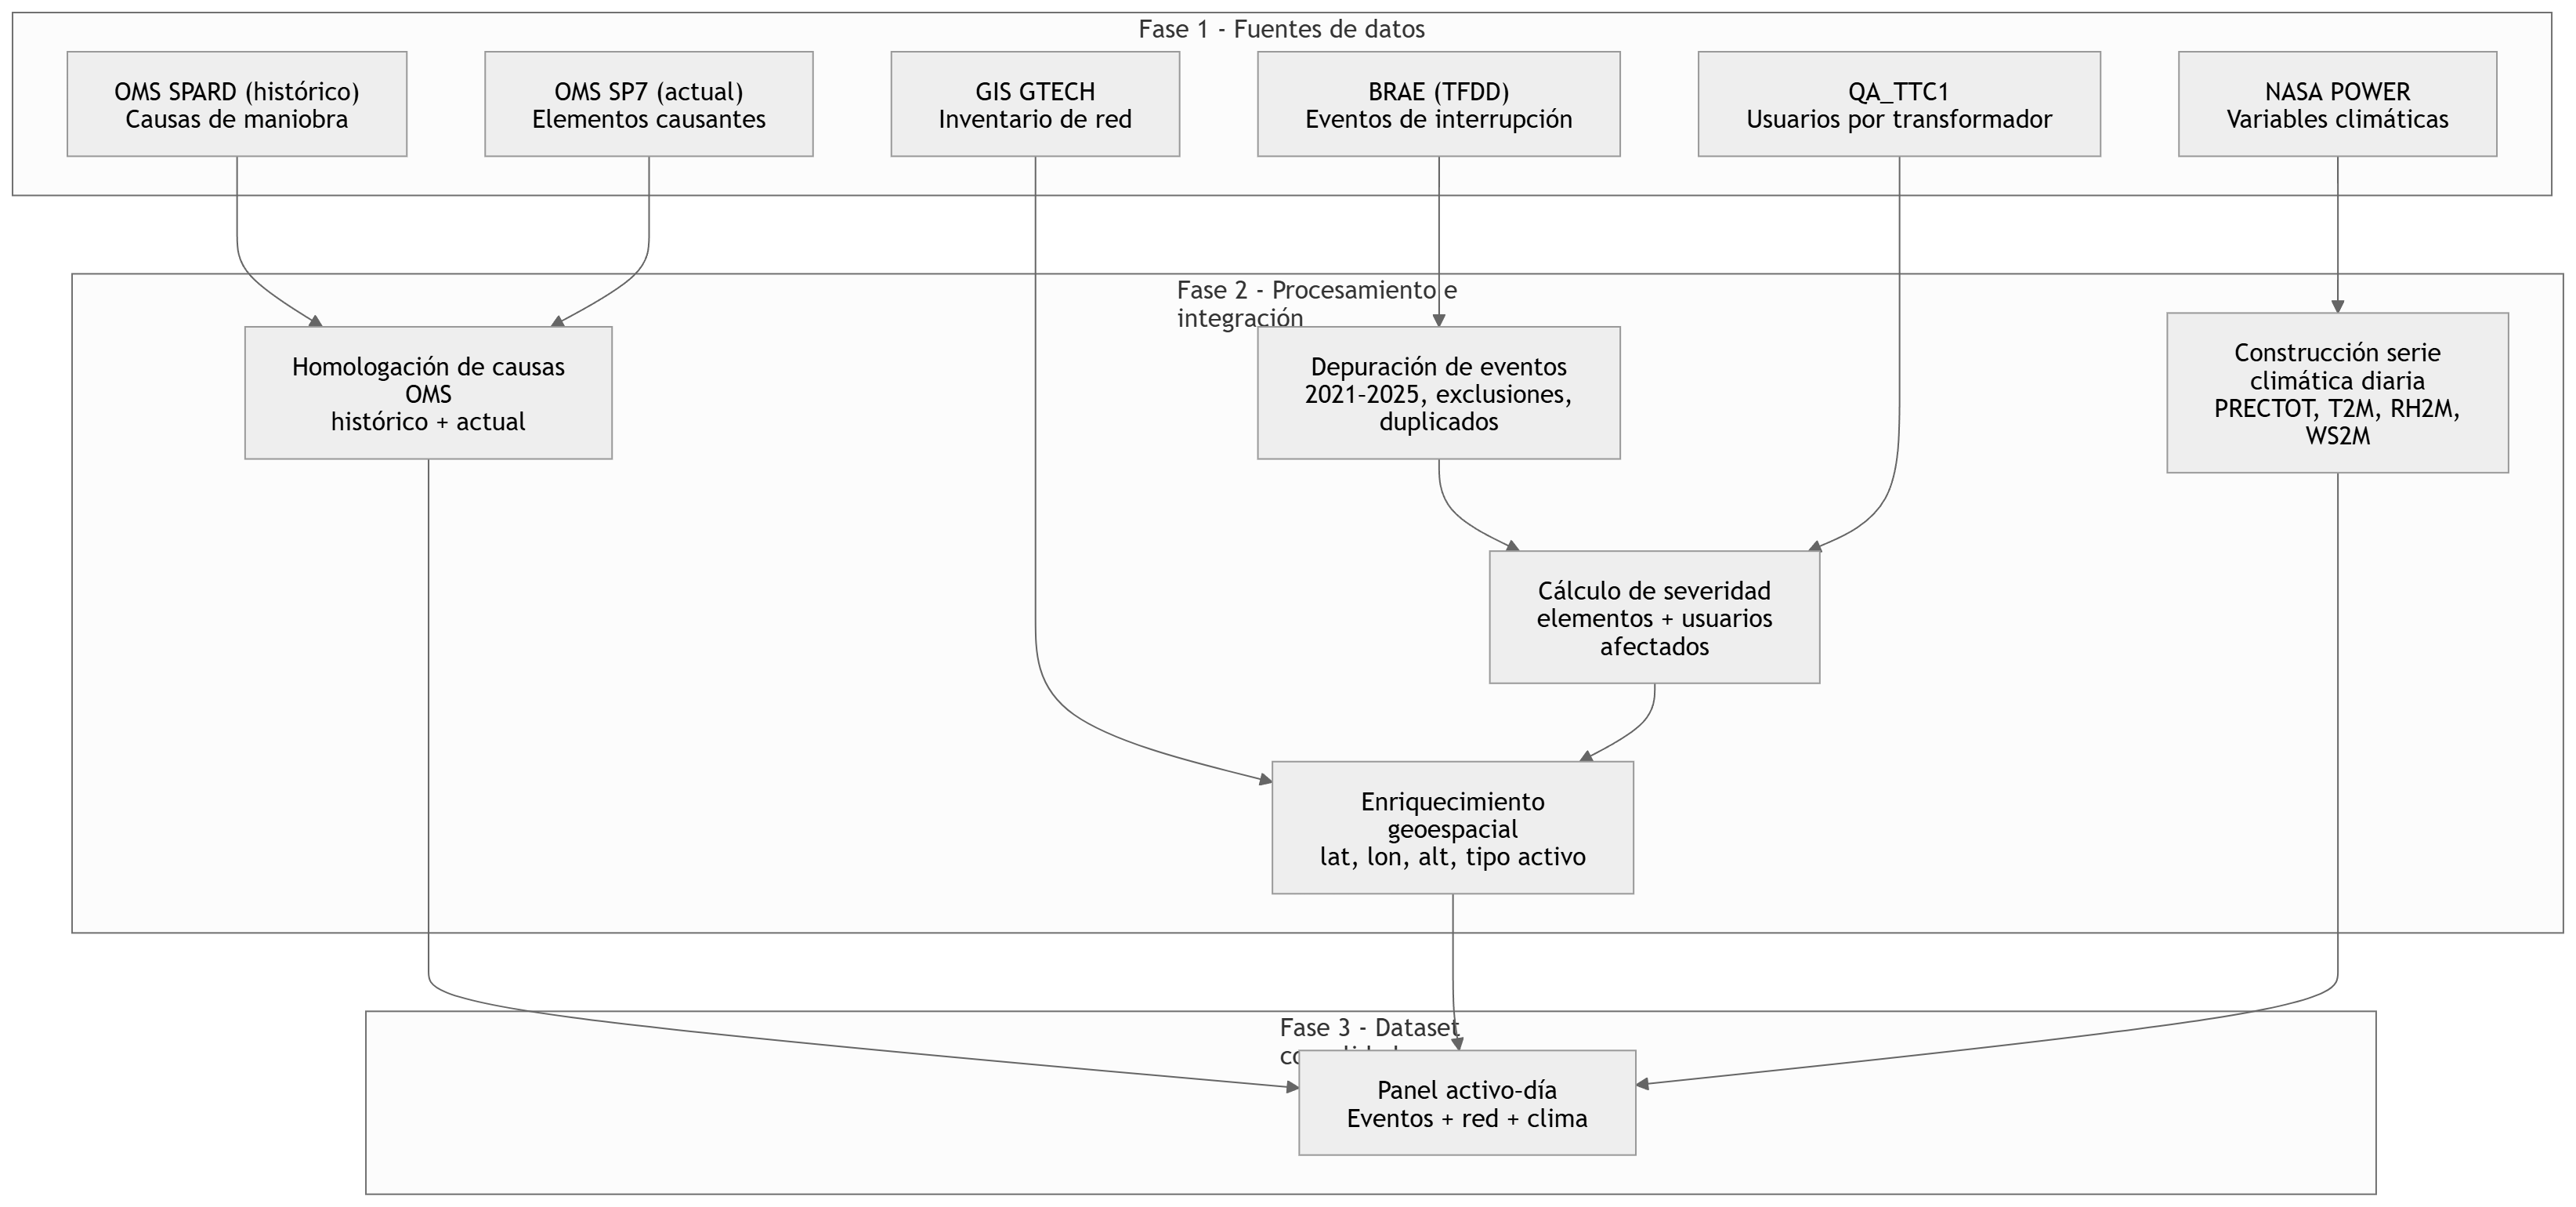
\includegraphics[width=1\textwidth]{img/drawings/mermaid-diagram (1).png}
    \caption{Estructura del panel de datos activo–día}
    \label{fig:panel_activo_dia}
\end{figure}


\subsection{Descripción de la tabla base consolidada}

Las Tablas~\ref{tab:muestra_consolidado_final_1} a~\ref{tab:muestra_consolidado_final_4} presentan una muestra de la tabla base consolidada resultante del paso~\ref{int:paso8}, con grano \textbf{activo eléctrico $\times$ día}. Por limitaciones de ancho en la página, la muestra se divide en cuatro bloques consecutivos que conservan el mismo orden de filas: identificación del activo (Tabla~\ref{tab:muestra_consolidado_final_1}), severidad y clima inicial (Tabla~\ref{tab:muestra_consolidado_final_2}), clima complementario (Tabla~\ref{tab:muestra_consolidado_final_3}) y variables de continuidad (Tabla~\ref{tab:muestra_consolidado_final_4}).

\begin{table}[H]
\centering
\small
\caption{Muestra de la tabla base consolidada (grano activo--día) -- Parte 1: activo y fecha}
\label{tab:muestra_consolidado_final_1}
\begin{tabular}{l l r r r l}
\toprule
\textbf{ID ACTIVO} & \textbf{TIPO} & \textbf{LAT.} & \textbf{LON.} & \textbf{ALT.} & \textbf{FECHA DIA} \\
\midrule
AASW4819 & Aisladero      & 8.5786778 & -72.92349 & 219  & 01/01/2021 \\
1T12452  & Transformador  & 8.5839989 & -72.92248 & 241  & 01/01/2021 \\
REC21365 & Reconectador   & 8.5840628 & -72.92246 & 241  & 01/01/2021 \\
CUC12345 & Cuchilla       & 7.7523729 & -73.23971 & 1236 & 01/01/2021 \\
INT39845 & Interruptor    & 7.7476080 & -73.25551 & 1359 & 02/01/2021 \\
AASW4820 & Aisladero      & 7.7561057 & -73.26037 & 1169 & 02/01/2021 \\
1T12453  & Aisladero      & 7.7409332 & -73.20825 & 1636 & 02/01/2021 \\
REC21366 & Transformador  & 7.7428641 & -73.18990 & 1542 & 02/01/2021 \\
CUC12346 & Reconectador   & 7.7538839 & -73.17721 & 1707 & 03/01/2021 \\
\bottomrule
\end{tabular}
\end{table}

\begin{table}[H]
\centering
\small
\caption{Muestra de la tabla base consolidada (grano activo--día) -- Parte 2: severidad y clima inicial (continuación)}
\label{tab:muestra_consolidado_final_2}
\begin{tabular}{l l r r r r}
\toprule
\textbf{ID ACTIVO} & \textbf{FECHA DIA} & \textbf{C. ELEM.} & \textbf{C. USU.} & \textbf{VEL. VIENTO} & \textbf{TEMP. MED.} \\
\midrule
AASW4819 & 01/01/2021 & 0   & 0    & 1.11 & 23.91 \\
1T12452  & 01/01/2021 & 0   & 0    & 1.23 & 24.58 \\
REC21365 & 01/01/2021 & 125 & 2015 & 0.96 & 23.04 \\
CUC12345 & 01/01/2021 & 0   & 0    & 0.81 & 23.02 \\
INT39845 & 02/01/2021 & 0   & 0    & 1.05 & 23.83 \\
AASW4820 & 02/01/2021 & 0   & 0    & 1.12 & 24.08 \\
1T12453  & 02/01/2021 & 0   & 0    & 1.08 & 24.52 \\
REC21366 & 02/01/2021 & 0   & 0    & 1.26 & 24.37 \\
CUC12346 & 03/01/2021 & 0   & 0    & 1.41 & 24.34 \\
\bottomrule
\end{tabular}
\end{table}

\begin{table}[H]
\centering
\small
\caption{Muestra de la tabla base consolidada (grano activo--día) -- Parte 3: clima complementario (continuación)}
\label{tab:muestra_consolidado_final_3}
\begin{tabular}{l l r r r r}
\toprule
\textbf{ID ACTIVO} & \textbf{FECHA DIA} & \textbf{HUM. REL.} & \textbf{TEMP. MIN.} & \textbf{TEMP. MAX.} & \textbf{PRECIP.} \\
\midrule
AASW4819 & 01/01/2021 & 78.91 & 20.06 & 29.98 & 3.19 \\
1T12452  & 01/01/2021 & 75.79 & 20.27 & 30.90 & 1.31 \\
REC21365 & 01/01/2021 & 83.94 & 20.26 & 27.82 & 3.19 \\
CUC12345 & 01/01/2021 & 79.55 & 17.92 & 30.09 & 7.28 \\
INT39845 & 02/01/2021 & 69.70 & 19.35 & 30.79 & 1.99 \\
AASW4820 & 02/01/2021 & 61.99 & 17.20 & 30.81 & 0.98 \\
1T12453  & 02/01/2021 & 72.16 & 20.38 & 30.59 & 2.70 \\
REC21366 & 02/01/2021 & 75.50 & 20.18 & 30.63 & 3.29 \\
CUC12346 & 03/01/2021 & 74.34 & 20.40 & 30.43 & 1.86 \\
\bottomrule
\end{tabular}
\end{table}

\begin{table}[H]
\centering
\small
\caption{Muestra de la tabla base consolidada (grano activo--día) -- Parte 4: variables de continuidad (continuación)}
\label{tab:muestra_consolidado_final_4}
\begin{tabular}{r r}
\toprule
\textbf{DURACION} & \textbf{FRECUENCIA} \\
\midrule
0     & 0 \\
0     & 0 \\
4.215 & 3 \\
0     & 0 \\
0     & 0 \\
0     & 0 \\
0     & 0 \\
0     & 0 \\
0     & 0 \\
\bottomrule
\end{tabular}
\end{table}

\noindent\textit{Nota:} las filas de las Tablas~\ref{tab:muestra_consolidado_final_1} a~\ref{tab:muestra_consolidado_final_4} corresponden al mismo conjunto de observaciones en el mismo orden. Los registros sin interrupción en el día presentan \texttt{DURACION = 0} y \texttt{FRECUENCIA = 0}.

\subsection{Descripción de las variables}

La Tabla~\ref{tab:muestra_consolidado_final_1} reúne las variables de identificación del activo y del periodo de observación. A continuación se describe el significado, origen, unidad y clasificación estadística de cada columna. Cada variable se clasifica como \textbf{cuantitativa} o \textbf{cualitativa}; en las cualitativas se distingue si la escala es \textbf{ordinal} o \textbf{categórica} (nominal). En las cuantitativas se indica además si la medición es \textbf{discreta} o \textbf{continua}. La Tabla~\ref{tab:clasificacion_variables} sintetiza esta clasificación para todas las variables del panel consolidado.

\begin{table}[H]
\centering
\small
\caption{Clasificación estadística de las variables del panel consolidado}
\label{tab:clasificacion_variables}
\begin{tabularx}{0.85\textwidth}{
>{\raggedright\arraybackslash}p{5.5cm}
>{\raggedright\arraybackslash}X
}
\toprule
\textbf{Variable} & \textbf{Clasificación} \\
\midrule
ID ACTIVO & Cualitativa categórica \\
TIPO & Cualitativa categórica \\
LAT., LON., ALT. & Cuantitativa continua \\
FECHA DIA & Cualitativa ordinal \\
C. ELEM., C. USU., FRECUENCIA & Cuantitativa discreta \\
VEL. VIENTO, TEMP. MED./MIN./MAX., HUM. REL., PRECIP., DURACION & Cuantitativa continua \\
\bottomrule
\end{tabularx}
\end{table}

\begin{itemize}
    \item \textbf{ID ACTIVO} (\texttt{ELEMENTO}): identificador único del activo eléctrico en la red de distribución. Proviene del inventario georreferenciado GIS (Sección~5.1.6, Tabla~5.5) y constituye la llave primaria del panel a nivel de activo. Permite vincular cada observación diaria con el elemento físico asociado a eventos de interrupción y con sus atributos espaciales. \textbf{Clasificación:} cualitativa categórica.

    \item \textbf{TIPO}: clasificación funcional del activo según su rol en la red. Los valores observados incluyen \emph{Transformador}, \emph{Reconectador}, \emph{Aisladero}, \emph{Cuchilla} e \emph{Interruptor}, homologados en la extracción GIS para estandarizar la tipología dentro del dataset consolidado. \textbf{Clasificación:} cualitativa categórica.

    \item \textbf{LAT.} (\texttt{LATITUD}): coordenada de latitud del activo, expresada en grados decimales (WGS84). Se obtiene del campo \texttt{coor\_gps\_lat} del sistema GTECH y habilita el análisis espacial de la red y la asignación de contexto geográfico a cada registro. \textbf{Clasificación:} cuantitativa continua.

    \item \textbf{LON.} (\texttt{LONGITUD}): coordenada de longitud del activo, expresada en grados decimales (WGS84). Corresponde al campo \texttt{coor\_gps\_lon} del inventario GIS y se emplea conjuntamente con la latitud para localizar el activo en el territorio de operación. \textbf{Clasificación:} cuantitativa continua.

    \item \textbf{ALT.} (\texttt{ALTITUD}): cota del activo sobre el nivel del mar, en metros. Proviene del campo \texttt{coor\_z} del sistema GIS y complementa la caracterización geográfica del punto de conexión en la red. \textbf{Clasificación:} cuantitativa continua.

    \item \textbf{FECHA DIA} (\texttt{FECHA\_DIA}): fecha calendario de la observación, con granularidad diaria en el intervalo 2021-01-01 a 2025-12-31. Se genera mediante el cruce del inventario de activos con el calendario diario (paso~\ref{int:paso4}) y define, junto con \texttt{ID ACTIVO}, la unidad muestral del panel \textbf{activo $\times$ día}. \textbf{Clasificación:} cualitativa ordinal.
\end{itemize}

\paragraph{Tabla~\ref{tab:muestra_consolidado_final_2} (severidad y clima inicial).}
Las columnas \texttt{ID ACTIVO} y \texttt{FECHA DIA} se repiten en esta tabla para facilitar la trazabilidad de filas entre bloques consecutivos. Las variables propias de este bloque son:

\begin{itemize}
    \item \textbf{C. ELEM.} (\texttt{CANTIDAD\_ELEMENTOS}): número de elementos de red afectados por el evento de interrupción asociado al activo en el día. Proviene de la Tabla~5.2 (afectación por evento, Sección~5.1.3) e integra al panel en el paso~\ref{int:paso5}. Cuando el activo no registra falla en el día, el valor es 0. \textbf{Clasificación:} cuantitativa discreta.

    \item \textbf{C. USU.} (\texttt{CANTIDAD\_USUARIOS}): número de usuarios afectados por el evento de interrupción vinculado al activo en el día. Se obtiene de la misma fuente y mediante el mismo cruce que \texttt{CANTIDAD\_ELEMENTOS}, y constituye una medida de severidad operativa del impacto sobre la demanda. En días sin interrupción, el valor es 0. \textbf{Clasificación:} cuantitativa discreta.

    \item \textbf{VEL. VIENTO} (\texttt{WS2M}): velocidad del viento a 2\,m de altura, expresada en m/s. Corresponde a la variable \texttt{WS2M} de NASA POWER (Sección~5.1.7) e integra al panel por \texttt{FECHA\_DIA} en el paso~\ref{int:paso6}. \textbf{Clasificación:} cuantitativa continua.

    \item \textbf{TEMP. MED.} (\texttt{T2M}): temperatura media del aire en el día, expresada en \textdegree C. Proviene del parámetro \texttt{T2M} de NASA POWER y captura las condiciones térmicas promedio del entorno asociadas a cada observación activo--día. \textbf{Clasificación:} cuantitativa continua.
\end{itemize}

\paragraph{Tabla~\ref{tab:muestra_consolidado_final_3} (clima complementario).}
Al igual que en la Tabla~\ref{tab:muestra_consolidado_final_2}, \texttt{ID ACTIVO} y \texttt{FECHA DIA} permiten alinear filas entre tablas. Las variables climáticas restantes del bloque son:

\begin{itemize}
    \item \textbf{HUM. REL.} (\texttt{RH2M}): humedad relativa del aire a 2\,m, expresada en porcentaje (\%). Proviene del parámetro \texttt{RH2M} de NASA POWER e integra al panel por \texttt{FECHA\_DIA}. \textbf{Clasificación:} cuantitativa continua.

    \item \textbf{TEMP. MIN.} (\texttt{T2M\_MIN}): temperatura mínima diaria del aire, expresada en \textdegree C. Corresponde al parámetro \texttt{T2M\_MIN} de NASA POWER y complementa la temperatura media con el extremo inferior del rango térmico del día. \textbf{Clasificación:} cuantitativa continua.

    \item \textbf{TEMP. MAX.} (\texttt{T2M\_MAX}): temperatura máxima diaria del aire, expresada en \textdegree C. Proviene del parámetro \texttt{T2M\_MAX} de NASA POWER y representa el extremo superior del rango térmico observado en el día. \textbf{Clasificación:} cuantitativa continua.

    \item \textbf{PRECIP.} (\texttt{PRECTOT}): precipitación total acumulada en el día, expresada en mm. Corresponde al parámetro \texttt{PRECTOT} de NASA POWER y permite incorporar la exposición del activo a condiciones de lluvia en la fecha de observación. \textbf{Clasificación:} cuantitativa continua.
\end{itemize}

\paragraph{Tabla~\ref{tab:muestra_consolidado_final_4} (variables de continuidad).}
Este bloque concentra las variables objetivo del análisis, construidas en el paso~\ref{int:paso7} a partir de la Tabla~5.1 (eventos depurados, Sección~5.1.2) y de los campos \texttt{FECHA\_DESCONEXION} y \texttt{FECHA\_CONEXION}:

\begin{itemize}
    \item \textbf{DURACION}: suma de horas sin servicio del activo efectivamente transcurridas en \texttt{FECHA\_DIA}. Si una interrupción cruza la medianoche, la duración total se prorratea entre los días calendario en los que el activo permaneció desconectado. En días sin falla, el valor es 0. \textbf{Clasificación:} cuantitativa continua.

    \item \textbf{FRECUENCIA}: número de interrupciones del activo cuyo inicio (\texttt{FECHA\_DESCONEXION}) ocurre en \texttt{FECHA\_DIA}. La frecuencia se contabiliza únicamente en el día de ocurrencia del evento, aun cuando la interrupción se extienda a días posteriores; en esos casos, la duración continúa distribuyéndose en los días sucesivos mediante la regla de \texttt{DURACION}. En días sin falla, el valor es 0. \textbf{Clasificación:} cuantitativa discreta.
\end{itemize}



\textbf{Objetivo específico asociado: OE1}

Una vez construido el panel consolidado, se aplican procedimientos de depuración y preprocesamiento sobre el dataset resultante. En esta fase se identifican datos faltantes, inconsistencias y valores atípicos que puedan afectar la calidad analítica del panel. Las actividades de preprocesamiento descritas a continuación preceden al análisis exploratorio (Etapa~3) y preparan el insumo base para la ingeniería de variables (Etapa~4).

Las actividades de preprocesamiento desarrolladas en esta etapa se describen en las subsecciones siguientes.

\subsection{Identificación de datos faltantes}

\subsection{Tratamiento de valores extremos en variables cuantitativas}


\subsection{Evidencia de calidad y confiabilidad de las fuentes}

La validación de los datos recopilados por Centrales Eléctricas de Norte de Santander S.A. E.S.P. (CENS) se fundamenta en su arquitectura institucional de gestión, enmarcada en la Política de Gestión de Tecnología de la Información (Sesión de la Junta Directiva No.~800 del 20 de febrero de 2018)~\cite{ref38} y en la Política del Sistema de Gestión Integrado (Sesión de la Junta Directiva No.~831 del 22 de abril de 2020)~\cite{ref2}, orientadas a garantizar una gestión sistemática de calidad continua, sostenibilidad ambiental y cumplimiento legal mediante la evaluación permanente de la calidad de los datos, priorizando consistencia, disponibilidad y accesibilidad de la información~\cite{ref39}.

CENS refuerza su gobernanza de datos mediante Instrumentos de Gestión de Información Pública, entre los cuales se destacan el Registro de Activos de Información (IPR), utilizado para detectar, clasificar y almacenar conjuntos de datos institucionales; los Cuadros de Clasificación Documental; el Esquema de Publicación de Información (IPS); el Índice de Información Clasificada y Reservada; los Costos de Reproducción; y el Programa de Gestión Documental (PGD). Estos instrumentos enmarcan el proceso institucional de almacenamiento, organización, acceso, difusión, protección y preservación de la información~\cite{ref40}.

En conjunto, estos mecanismos reflejan sistemas de control interno, gobernanza, confianza en la información documentada y transparencia institucional. Asimismo, evidencian el funcionamiento estructurado de los registros y su disponibilidad operativa, garantizando la calidad, veracidad y consistencia de los datos utilizados en este estudio para la toma de decisiones analíticas y gerenciales.

La fiabilidad técnica de las fuentes climáticas y ambientales está respaldada por el IDEAM, entidad pública responsable de la recopilación oficial de datos hidrológicos, meteorológicos y ambientales en Colombia. El IDEAM opera bajo la Política Institucional para la Gestión de Información Estadística (E-SGI-PI003)~\cite{ref41} y las disposiciones del Sistema Estadístico Nacional, que establecen normas obligatorias de trazabilidad, control de calidad, validación estadística, metadatos estructurados y consistencia metodológica en los procesos de captura, procesamiento y difusión de datos~\cite{ref42}.

Adicionalmente, en cumplimiento del Decreto 1081 de 2015, el Decreto 103 de 2015, la Ley 1712 de 2014 (Ley de Transparencia) y la Resolución 1519 de 2020 del MINTIC, el IDEAM garantiza que la información publicada sea auditable, actualizada y accesible, respaldada por canales institucionales de difusión, monitoreo interno e integridad documental. Estas disposiciones fortalecen la calidad estadística y aseguran que las series climáticas oficiales cumplan criterios formales de confiabilidad, oportunidad y validez técnica a escala nacional~\cite{ref41,ref42,ref43}.


\section{Etapa 3 – Análisis descriptivo y exploratorio de datos (EDA)}

\textbf{Objetivo específico asociado: OE2}

\textbf{Objetivo:} comprender el comportamiento de los datos e identificar patrones, relaciones y comportamientos relevantes que orienten las decisiones de modelado.

Una vez completadas las etapas de extracción, integración y preprocesamiento, se desarrolla un análisis exploratorio orientado a caracterizar las distribuciones de las variables, identificar patrones temporales y espaciales, y evaluar las relaciones entre covariables que podrían explicar la variación de $SAIDI$ y $SAIFI$. Esta etapa se concibe como un análisis diagnóstico previo al modelamiento, orientado a garantizar la estabilidad e interpretabilidad de los resultados.

Para las variables cuantitativas se calculan medidas de tendencia central y dispersión, así como la proporción de valores atípicos; adicionalmente se construyen histogramas y diagramas de caja para examinar la forma de las distribuciones. En el caso de las variables categóricas, se analizan las frecuencias absolutas y relativas de cada categoría. El grado de asociación entre variables cuantitativas se evalúa mediante el coeficiente de correlación de Spearman y entre variables cualitativas mediante el estadístico de Cramér, con el fin de identificar redundancias y relaciones preliminares que orienten la depuración de variables en la Etapa~4. Las visualizaciones incluyen series de tiempo, gráficos de dispersión, mapas temáticos y mapas de calor de correlaciones.


Las actividades desarrolladas en esta etapa se describen en las subsecciones siguientes.

\subsection{Caracterización del panel consolidado}

\subsection{Cálculo de estadísticos descriptivos}

\subsection{Análisis de la distribución de variables}

\subsection{Análisis temporal de eventos}

\subsection{Identificación de patrones y tendencias}

\subsection{Visualización exploratoria}

\subsection{Análisis de correlación y asociación}

\subsection{Evaluación inicial de relaciones multivariadas}

\subsection{Segmentación exploratoria}

\subsection{Identificación de comportamiento atípico}

\subsection{Resultados y entregables de la etapa}


\textbf{Resultado:} conocimiento exploratorio del comportamiento de los datos y hallazgos relevantes para el modelado.

\textbf{Entregable:} Documento de análisis descriptivo y exploratorio (EDA).


\section{Etapa 4 – Ingeniería de variables y preparación del modelo}

\textbf{Objetivo específico asociado: OE2}

\textbf{Objetivo:} construir las variables analíticas necesarias para el entrenamiento de modelos predictivos, asegurando un dataset consistente, balanceado y estadísticamente apto para la modelación.

A partir de los hallazgos del EDA, en esta etapa se transforma el dataset consolidado en una representación analítica adecuada para el entrenamiento de modelos. Esto incluye la definición formal de la variable respuesta, la construcción de variables predictoras informadas por el comportamiento observado, la depuración y codificación de covariables, la estandarización de variables continuas y la definición de las particiones temporales de entrenamiento y prueba. El preprocesamiento orientado al modelado ---incluida la selección de variables con base en los análisis de asociación del EDA--- se concentra en esta etapa, en coherencia con criterios de estabilidad numérica, identificabilidad del modelo y validez de supuestos.

Las actividades desarrolladas en esta etapa se describen en las subsecciones siguientes.

\subsection{Construcción de variables predictoras}

\subsection{Construcción de la variable respuesta}

\subsection{Análisis de asociación y depuración de variables cuantitativas}

\subsection{Análisis de asociación y depuración de variables cualitativas}

\subsection{Codificación de variables categóricas}

\subsection{Estandarización de variables cuantitativas}

\subsection{Generación de ventanas temporales}

\subsection{Partición de datos en entrenamiento y prueba}

\subsection{Construcción de matrices de diseño}

\subsection{Reducción de dimensionalidad}

\subsection{Segmentación analítica}

\subsection{Transformaciones adicionales para modelado}

\subsection{Resultados y entregables de la etapa}

\textbf{Resultado:} dataset analítico listo para entrenamiento y validación del modelo.

\textbf{Entregable:} Reporte técnico de ingeniería de variables y dataset analítico documentado.


\section{Etapa 5 – Modelado predictivo y evaluativo}

\textbf{Objetivo específico asociado: OE2 y OE3}

\textbf{Objetivo:} entrenar, validar y evaluar modelos predictivos utilizando métricas de desempeño que permitan estimar $SAIDI$ y $SAIFI$ por circuito o área.

En esta etapa se desarrollan y evalúan diversos modelos estadísticos y de aprendizaje automático. La selección del enfoque (supervisado, no supervisado o híbrido) se determina según los hallazgos del análisis exploratorio, la naturaleza de los datos disponibles y los requerimientos de interpretabilidad. La evaluación comparativa considera métricas de error como $RMSE$, $MAE$ y $MAPE$, así como la estabilidad del modelo y la validez de supuestos. Adicionalmente, se realiza un análisis de importancia de variables mediante técnicas interpretables, con el objetivo de identificar los factores operativos, técnicos o climáticos que influyen de manera significativa en la calidad del servicio.

Las actividades desarrolladas en esta etapa se describen en las subsecciones siguientes.

\subsection{Selección de algoritmos}

\subsection{Entrenamiento del modelo}

\subsection{Validación del modelo}

\subsection{Ajuste de hiperparámetros}

\subsection{Evaluación de desempeño}

\subsection{Comparación de modelos}

\subsection{Interpretación de resultados}

\subsection{Resultados y entregables de la etapa}

\textbf{Resultado:} modelo predictivo validado y evaluado técnicamente.

\textbf{Entregables:} Informe de evaluación comparativa de modelos predictivos (OE3) y reporte técnico de importancia de variables (OE2).


\section{Etapa 6 – Cierre metodológico, documentación y reportes}

\textbf{Objetivo específico asociado: OE1–OE2–OE3}

\textbf{Objetivo:} presentar los resultados obtenidos y documentar el proceso metodológico desarrollado, asegurando la reproducibilidad y la trazabilidad de los hallazgos.

En la etapa final se consolidan los resultados del proyecto y se documentan de forma integral las técnicas aplicadas, las transformaciones realizadas y el código reproducible (en R o Python). El capítulo incluye apéndices técnicos, tablas de validación, bibliografía y lineamientos de reproducibilidad, así como una discusión orientada a interpretar los hallazgos en términos técnicos y operativos para la toma de decisiones del operador de red.

Las actividades desarrolladas en esta etapa se describen en las subsecciones siguientes.

\subsection{Presentación de resultados del modelo}

\subsection{Métricas de desempeño}

\subsection{Hallazgos principales}

\subsection{Interpretación técnica y operativa}

\subsection{Generación de reportes}

\subsection{Discusión de resultados}

\subsection{Limitaciones y trabajos futuros}

\subsection{Resultados y entregables de la etapa}

\textbf{Resultado:} documentación final del proyecto y resultados consolidados.

\textbf{Entregables:} Compendio de documentación del proyecto (informe final, informe descriptivo, informe de evaluación de modelos y reporte técnico de variables relevantes), código reproducible y documentación detallada de procesos y transformaciones.
   

%--------------------------------------------------

    
    

     % --------------------------
     \chapter{Resultados}
     %--------------------------------------------------

\section{Etapa 1}
\label{sec:resultados-etapa1}



\section{Etapa 2}
\label{sec:resultados-etapa2}




\section{Etapa 3}
\label{sec:resultados-etapa3}




\section{Etapa 4}
\label{sec:resultados-etapa4}



\section{Etapa 5}
\label{sec:resultados-etapa5}



\section{Etapa 6}
\label{sec:resultados-etapa6}
   
   
    
        
    
    % --------------------------
    \chapter{Discusión y trabajo futuro}
    
%--------------------------------------------------
\section{Discusión}

\label{sec:discusion}

\begin{itemize}
    \item Objetivo 1: 
    \item Objetivo 2:
    \item Objetivo 3:
    \item Objetivo 4:
\end{itemize}

%--------------------------------------------------
\section{Trabajos futuros}



   % --------------------------
    \chapter{Conclusiones}
    
\section{Conclusión asociada al objetivo general}

Este trabajo desarrolló y validó una metodología basada en ciencia de datos para pronosticar y explicar los indicadores SAIDI y SAIFI en la red de distribución de energía eléctrica de una empresa del Norte de Santander, a partir de la integración de seis fuentes de datos heterogéneas (BRAE, OMS SPARD/SP7, GIS, NASA POWER, más sismicidad, desastres y vegetación) en un panel único cuadrante--semana. La metodología combinó modelos de pronóstico semanal (Pooled OLS, efectos fijos y Random Forest) con modelos espaciales formales (SAR, SEM), obteniendo en ambos casos desempeños satisfactorios para sus respectivos propósitos: predicción bajo incertidumbre temporal real y explicación estructural del patrón territorial de calidad del servicio. El objetivo general se cumple en la medida en que el pipeline completo, desde la extracción de datos crudos hasta los modelos validados, quedó documentado de forma reproducible y aplicable por la empresa a su labor de gestión diaria de la red.

\section{Conclusión asociada al objetivo específico 1}

Se consolidó un repositorio analítico unificado y trazable a partir de seis fuentes complementarias, documentado mediante una tabla de linaje de datos (Tabla~\ref{tab:data_lineage}) que especifica, para cada fuente, las variables extraídas, el proceso de depuración aplicado y el resultado obtenido. El panel final no presenta valores faltantes ($0$~\% sobre $N_{\mathrm{agr}}=90{.}128$ observaciones cuadrante--semana), y el proceso de integración permitió identificar y documentar explícitamente una limitación de cobertura —un sesgo sistemático de emparejamiento evento--elemento durante 2021--2023— que de otro modo habría comprometido silenciosamente la calidad de los resultados. La delimitación consecuente del dataset de modelado a 2024--2025 constituye, en sí misma, una métrica de integridad aplicada: se prefirió un panel más corto pero confiable a uno más extenso con sesgo no controlado.

\section{Conclusión asociada al objetivo específico 2}

Las variables operativas, técnicas y climáticas más relevantes para predecir SAIDI y SAIFI, identificadas de forma convergente por la importancia de variables del Random Forest y por los coeficientes de los modelos espaciales SAR/SEM, corresponden principalmente a características de infraestructura y exposición territorial: el número de elementos de red y la longitud de red del cuadrante, la antigüedad del activo más viejo, la composición de estrato y de clientes no residenciales, y en menor medida la exposición sísmica y la vegetación (NDVI). En contraste, la señal climática contemporánea (temperatura, humedad, viento y precipitación de la misma semana) resultó comparativamente débil una vez controlada la redundancia entre variables climáticas correlacionadas (VIF reducido de un máximo de $43{.}92$ a $7{.}21$). Este hallazgo es relevante porque contradice la expectativa inicial de que el clima sería el principal predictor, y en cambio señala que la infraestructura de red —una variable sobre la que el operador tiene margen de gestión directa— es el factor más informativo disponible \emph{ex ante}.

\section{Conclusión asociada al objetivo específico 3}

Se evaluó el desempeño de seis métodos —cuatro de panel semanal (Pooled OLS, efectos fijos de cuadrante, efectos fijos de cuadrante y semana, Random Forest) y dos modelos espaciales formales (SAR, SEM)— para predecir SAIDI y SAIFI por cuadrante, considerando tanto la naturaleza de los datos como la interpretabilidad requerida por los gestores. Random Forest resultó el modelo de pronóstico semanal con menor error para SAIDI (RMSE $=0{.}1195$), mientras que el modelo de efectos fijos de cuadrante fue superior para SAIFI (RMSE $=0{.}0026$), evidenciando que no existe un método único óptimo para ambos indicadores. Para la explicación estructural, los modelos espaciales SAR (SAIDI) y SEM (SAIFI) resultaron preferidos por AIC sobre el corte transversal ponderado por cuadrante, con una capacidad explicativa alta cuantificada mediante su regresión lineal equivalente ($R^2 = 0{.}901$ y $R^2 = 0{.}837$, respectivamente), verificada mediante pruebas de robustez que descartan que dicha capacidad sea un artefacto de colinealidad. Estos resultados permiten recomendar de forma diferenciada, según el propósito operativo: Random Forest o efectos fijos de cuadrante para pronóstico de corto plazo, y SAR/SEM para el diagnóstico territorial estructural de la calidad del servicio.

   % --------------------------
    \clearpage
    \printbibliography
    % --------------------------
     \begin{appendices}
    \chapter{Appendix}
        
\section{Diagrama de integración del panel}
\label{app:diagrama_panel}

La Figura~\ref{fig:panel_activo_dia} presenta el diagrama de flujo de la secuencia de integración descrita en la Sección~\ref{sec:logica_integracion}, desde las fuentes de origen hasta el panel consolidado activo~$\times$~día.

\begin{figure}[!htbp]
    \centering
    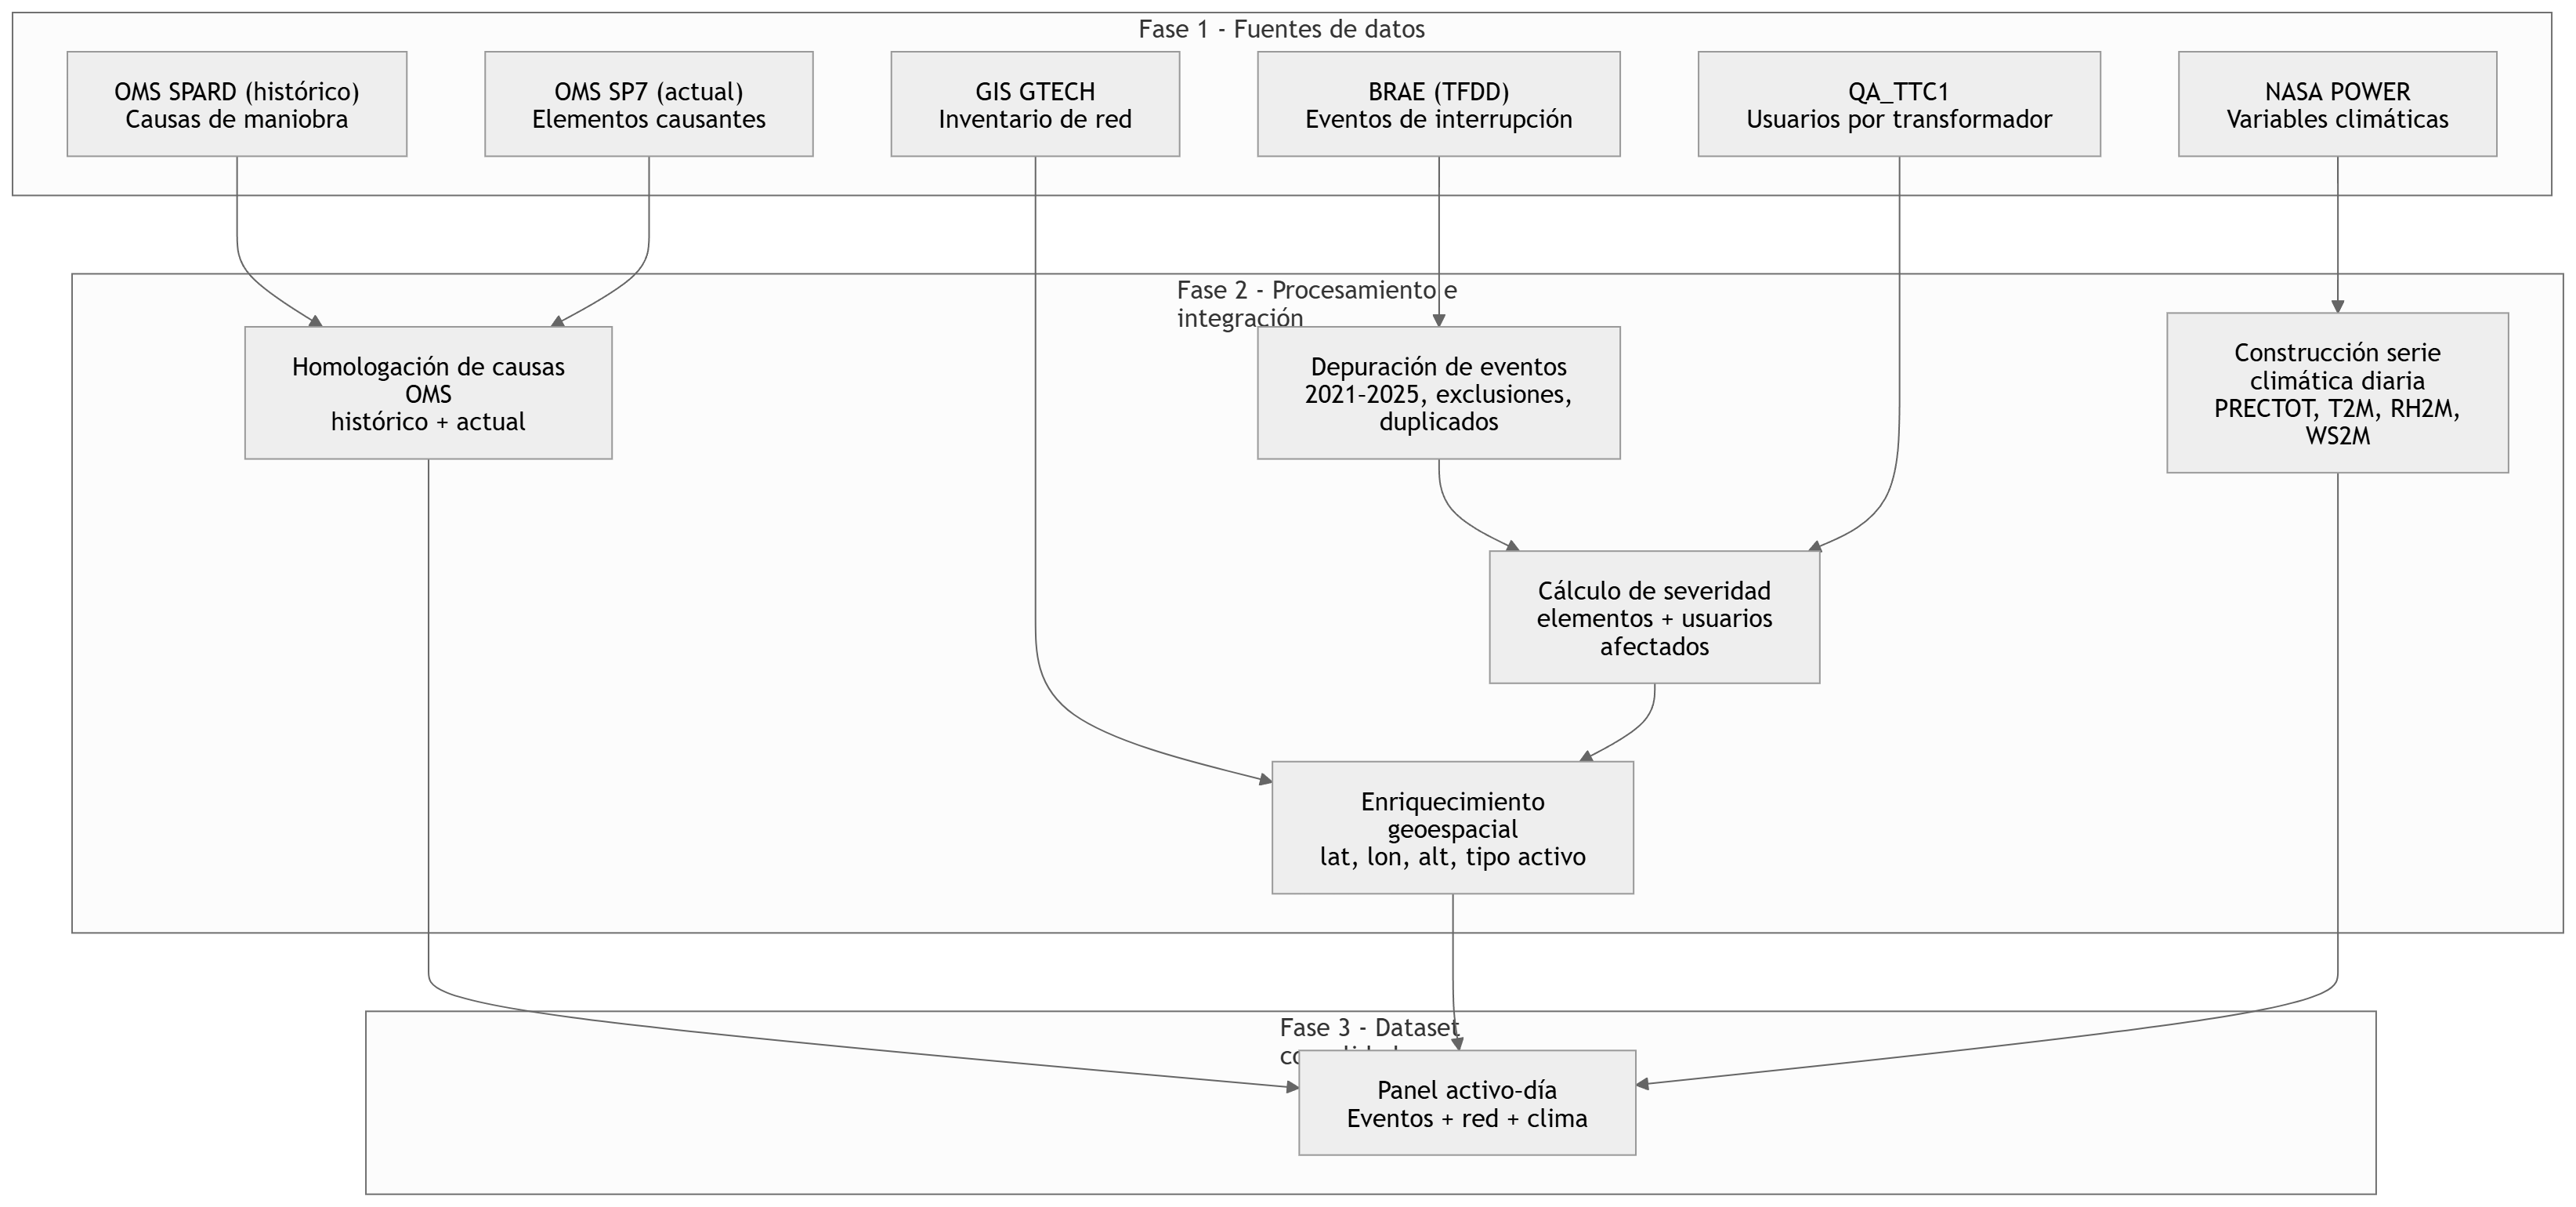
\includegraphics[width=\textwidth]{img/drawings/mermaid-diagram (1).png}
    \caption{Estructura del panel de datos activo–día}
    \label{fig:panel_activo_dia}
\end{figure}

\section{Código de extracción de datos}
\label{app:codigo}

Esta sección consolida el código de extracción utilizado en la Etapa~1 de la metodología (consultas SQL y fragmentos Python). En el cuerpo del documento se describe el procedimiento y se referencia el listado correspondiente.

\subsection{Consultas SQL}

\subsubsection{Eventos de interrupción (BRAE)}
\label{app:sql-brae}

\begin{lstlisting}[style=thesiscode,language=SQL,caption={Consulta SQL de extracción y depuración de eventos de interrupción (BRAE)},label={lst:sql_brae}]
SELECT DISTINCT FDD_CODIGOEVENTO AS ID_EVENTO
      ,FDD_FINICIAL AS FECHA_DESCONEXION
      ,FDD_FFINAL AS FECHA_CONEXION
      ,'' AS ELEMENTO_FALLADO
FROM BRAE.QA_TFDDREGISTRO
WHERE TO_CHAR(FDD_FINICIAL,'YYYY') IN ('2021', '2022', '2023', '2024', '2025')
  AND FDD_EXCLUSION = 'NO EXCLUIDA'
  AND FDD_CAUSA_SSPD NOT IN (1)
  AND FDD_FFINAL IS NOT NULL;
\end{lstlisting}

\subsubsection{Afectación por evento (BRAE + QA\_TTC1)}
\label{app:sql-afectacion}

\begin{lstlisting}[style=thesiscode,language=SQL,caption={Consulta SQL de afectación por evento (elementos y usuarios)},label={lst:sql_afectacion}]
SELECT FDD_CODIGOEVENTO AS ID_EVENTO
      ,COUNT(FDD_CODIGOELEMENTO) AS CANTIDAD_ELEMENTOS_FALLADOS
      ,SUM(CANTIDAD_USUARIOS) AS CANTIDAD_USUARIOS
FROM BRAE.QA_TFDDREGISTRO
LEFT JOIN (
    SELECT TC1_CODCONEX AS TRANSFORMADOR
          ,COUNT(TC1_CODCONEX) AS CANTIDAD_USUARIOS
          ,TC1_PERIODO AS PERIODO
    FROM QA_TTC1
    WHERE SUBSTR(TC1_PERIODO, 1, 4) IN ('2021', '2022', '2023', '2024', '2025')
    GROUP BY TC1_PERIODO, TC1_CODCONEX
) ON FDD_CODIGOELEMENTO = TRANSFORMADOR
 AND FDD_PERIODO_TC1 = PERIODO
WHERE TO_CHAR(FDD_FINICIAL,'YYYY') IN ('2021', '2022', '2023', '2024', '2025')
  AND FDD_EXCLUSION = 'NO EXCLUIDA'
  AND FDD_CAUSA_SSPD NOT IN (1)
  AND FDD_FFINAL IS NOT NULL
GROUP BY FDD_CODIGOEVENTO;
\end{lstlisting}

\subsubsection{Elemento causante histórico (OMS SPARD)}
\label{app:sql-oms-historico}

\begin{lstlisting}[style=thesiscode,language=SQL,caption={Consulta SQL del elemento causante histórico (OMS SPARD)},label={lst:sql_oms_historico}]
SELECT CODE AS CODIGO_MANIOBRA
      ,BREAKER AS ELEMENTO_FALLADO
FROM OMS.MANIOBRAS@SPARD
WHERE TO_NUMBER(TO_CHAR(FECHA, 'YYYY')) >= 2021
  AND CAUSA != 'PRUEBA';
\end{lstlisting}

\subsubsection{Inventario georreferenciado (GIS GTECH)}
\label{app:sql-gis}

\begin{lstlisting}[style=thesiscode,language=SQL,caption={Consulta SQL del inventario georreferenciado de activos (GIS GTECH)},label={lst:sql_gis}]
SELECT 
    nodo_transform_v AS ELEMENTO,
    coor_gps_lat     AS LATITUD,
    coor_gps_lon     AS LONGITUD,
    coor_z           AS ALTITUD,
    'Transformador'  AS TIPO,
    ubicacion
FROM ccomun@gtech c
JOIN cconectividad_e@gtech USING (g3e_fid)
WHERE c.estado = 'OPERACION'
  AND c.g3e_fno = 20400
UNION
SELECT 
    r.codigo         AS ELEMENTO,
    coor_gps_lat     AS LATITUD,
    coor_gps_lon     AS LONGITUD,
    coor_z           AS ALTITUD,
    'Reconectador'   AS TIPO,
    ubicacion
FROM ereconec_at@gtech r
JOIN ccomun@gtech c USING (g3e_fid)
JOIN cconectividad_e@gtech USING (g3e_fid)
WHERE c.estado = 'OPERACION';
\end{lstlisting}

\noindent La consulta del Listado~\ref{lst:sql_gis} se replica de forma análoga para Interruptor, Cuchilla, Aisladero, Reconectador y Transformador, homologando el tipo de activo en cada bloque \texttt{UNION}.

\subsection{Fragmentos Python}

\subsubsection{Elemento causante actual (OMS SP7)}
\label{app:py-oms-sp7}

\begin{lstlisting}[style=thesiscode,language=Python,caption={Fragmento Python de lectura y depuración del elemento causante actual (OMS SP7)},label={lst:py_oms_sp7}]
columnas_necesarias = ['Maniobra Apertura', 'Tipo Elemento', 'Elemento_Falla']
df = pd.read_csv(ruta_actual)
df.columns = df.columns.str.strip()
df = df[columnas_necesarias].drop_duplicates()
\end{lstlisting}

\subsubsection{Parámetros meteorológicos (NASA POWER)}
\label{app:py-nasa}

\begin{lstlisting}[style=thesiscode,language=Python,caption={Definición de parámetros meteorológicos extraídos de NASA POWER},label={lst:py_nasa}]
parametros_nasa = ("PRECTOT", "T2M", "T2M_MAX", "T2M_MIN", "RH2M", "WS2M")
\end{lstlisting}

\section{Informes reproducibles (HTML)}
\label{app:informes-html}

Los procedimientos de extracción, integración y análisis exploratorio descritos en la metodología se documentan de forma reproducible en informes HTML publicados en el repositorio del proyecto (GitHub Pages). En el cuerpo del documento se cita el apartado correspondiente de este apéndice; los hipervínculos a cada informe se concentran aquí.

\subsection{Consolidación del panel activo--día}
\label{app:html-consolidada}
Informe \texttt{Consolidada.html}: detalle de los pasos~\ref{paso:int-4} a~\ref{paso:int-8} de integración hacia el panel consolidado.
\href{\urlconsolidada}{Abrir informe}.

\subsection{Agrupación cuadrante $\times$ semana}
\label{app:html-agrupacion}
Informe \texttt{data\_agrupacion.html}: construcción de la tabla de análisis a grano cuadrante~$\times$~semana.
\href{\urlagrupacion}{Abrir informe}.

\subsection{Datos faltantes (tabla agrupada)}
\label{app:html-faltantes-agrupada}
Informe \texttt{missing\_values\_grouped.html}: diagnóstico de valores faltantes en \texttt{data\_agrupada.csv}.
\href{\urlfaltantesagrupada}{Abrir informe}.

\subsection{Valores extremos (panel consolidado)}
\label{app:html-outliers}
Informe \texttt{detection\_outliers.html}: identificación de valores extremos en el panel activo~$\times$~día.
\href{\urldetectionoutliers}{Abrir informe}.

\subsection{Valores extremos (tabla agrupada)}
\label{app:html-outliers-agrupada}
Informe \texttt{outliers\_gruped.html}: identificación de valores extremos en la tabla cuadrante~$\times$~semana.
\href{\urloutliersagrupada}{Abrir informe}.

\subsection{Estadísticos descriptivos}
\label{app:html-descriptivos}
Informe \texttt{calculo\_estadistico\_descriptivo.html}: cálculo de estadísticos descriptivos sobre la tabla agrupada.
\href{\urlestadisticosdescriptivos}{Abrir informe}.

\subsection{Distribución de variables}
\label{app:html-distribucion}
Informe \texttt{distribucion\_variables.html}: análisis de la forma de las distribuciones (densidades, asimetría, curtosis y ceros).
\href{\urldistribucionvariables}{Abrir informe}.

\subsection{Análisis temporal de eventos}
\label{app:html-temporal}
Informe \texttt{analisis\_temporal\_eventos.html}: series semanales, estacionalidad y autocorrelación de eventos.
\href{\urlanalisistemporal}{Abrir informe}.

\subsection{Emparejamiento evento--elemento}
\label{app:html-emparejamiento}
Informe \texttt{emparejamiento\_eventos.html}: cobertura anual de la trazabilidad entre eventos BRAE e inventario GIS.
\href{\urlemparejamientoeventos}{Abrir informe}.

\subsection{Materialización de $D_{\mathrm{mod}}$}
\label{app:html-datamod}
Informe \texttt{consolidado\_data\_mod.html}: filtro y exportación del dataset de modelado 2024--2025.
\href{\urlconsolidadodatamod}{Abrir informe}.

\subsection{Identificación de patrones}
\label{app:html-patrones}
Informe \texttt{identificacion\_patrones.html}: patrones temporales, espaciales y clima--evento sobre $D_{\mathrm{mod}}$.
\href{\urlidentificacionpatrones}{Abrir informe}.

\subsection{Análisis de correlación}
\label{app:html-correlacion}
Informe \texttt{analisis\_correlacion.html}: asociaciones de Spearman entre variables climáticas y operativas.
\href{\urlanalisisCorrelacion}{Abrir informe}.

\subsection{Análisis multivariado}
\label{app:html-multivariado}
Informe \texttt{analisis\_multivariado.html}: VIF, PCA, agrupamiento jerárquico y GLM Poisson exploratorio.
\href{\urlanalisisMultivariado}{Abrir informe}.

\subsection{Segmentación exploratoria}
\label{app:html-segmentacion}
Informe \texttt{segmentacion\_exploratoria.html}: perfiles por nivel de actividad, régimen de lluvia y clustering de cuadrantes.
\href{\urlsegmentacionexploratoria}{Abrir informe}.

\subsection{EDA consolidado}
\label{app:html-eda}
Informe \texttt{EDA.html}: síntesis ejecutiva del análisis exploratorio (Etapa~3) con hallazgos y lineamientos para la Etapa~4.
\href{\urlEDA}{Abrir informe}.

\subsection{Asociación y depuración de variables cuantitativas}
\label{app:html-asociacion-cuanti}
Informe \texttt{asociacion\_depuracion\_cuantitativas.html}: depuración \emph{ex ante} de covariables cuantitativas y exportación de la matriz de diseño.
\href{\urlasociaciondepuracioncuanti}{Abrir informe}.

\subsection{Justificación de la agregación espacial}
\label{app:html-etapa2-03}
Informe \texttt{Etapa2\_03\_justificacion\_agregacion\_espacial.html}: justificación del grano cuadrante~$\times$~semana y evidencia de concentración espacial de fallas.
\href{\urlEtapaDosTres}{Abrir informe}.

\subsection{Infraestructura eléctrica por cuadrante}
\label{app:html-etapa2-04}
Informe \texttt{Etapa2\_04\_infraestructura\_gis\_cuadrante.html}: agregación de tipologías y conteos de infraestructura GIS al polígono de cada cuadrante.
\href{\urlEtapaDosCuatro}{Abrir informe}.

\subsection{Estratificación municipal}
\label{app:html-etapa2-05}
Informe \texttt{Etapa2\_05\_estratificacion\_municipal.html}: asignación espacial de municipio y estrato predominante a cuadrantes reales.
\href{\urlEtapaDosCinco}{Abrir informe}.

\subsection{Eventos catastróficos UNGRD}
\label{app:html-etapa2-06}
Informe \texttt{Etapa2\_06\_desastres\_ungrd.html}: integración de emergencias UNGRD a municipio/cuadrante y semana.
\href{\urlEtapaDosSeis}{Abrir informe}.

\subsection{Sismicidad SGC}
\label{app:html-etapa2-07}
Informe \texttt{Etapa2\_07\_sismicidad\_sgc.html}: incorporación de sismicidad del SGC como exposición territorial del panel.
\href{\urlEtapaDosSiete}{Abrir informe}.

\subsection{Topología de red eléctrica}
\label{app:html-etapa2-08}
Informe \texttt{Etapa2\_08\_topologia\_red.html}: métricas topológicas de red por cuadrante y vecindad espacial/eléctrica.
\href{\urlEtapaDosOcho}{Abrir informe}.

\subsection{Integración del panel final}
\label{app:html-etapa2-09}
Informe \texttt{Etapa2\_09\_integracion\_panel\_final.html}: unión de fuentes enriquecidas hacia el panel base de modelado.
\href{\urlEtapaDosNueve}{Abrir informe}.

\subsection{Cargue NASA POWER semanal}
\label{app:html-etapa2-10}
Informe \texttt{Etapa2\_10\_cargue\_nasa\_semana.html}: cargue de variables climáticas NASA POWER agregadas por semana.
\href{\urlEtapaDosDiez}{Abrir informe}.

\subsection{Cargue de eventos semanales}
\label{app:html-etapa2-11}
Informe \texttt{Etapa2\_11\_cargue\_eventos\_semana.html}: agregación de eventos y métricas de continuidad a cuadrante--semana.
\href{\urlEtapaDosOnce}{Abrir informe}.

\subsection{Unión del panel semanal}
\label{app:html-etapa2-12}
Informe \texttt{Etapa2\_12\_union\_panel\_semana.html}: unión semanal de clima, eventos y atributos territoriales.
\href{\urlEtapaDosDoce}{Abrir informe}.

\subsection{Modelo espacial de SAIDI}
\label{app:html-etapa5-01}
Informe \texttt{Etapa5\_01\_modelo\_SAIDI\_espacial.html}: estimación, validación e interpretación del modelo espacial de SAIDI.
\href{\urlEtapaCincoUno}{Abrir informe}.

\subsection{Modelo espacial de SAIFI}
\label{app:html-etapa5-02}
Informe \texttt{Etapa5\_02\_modelo\_SAIFI\_espacial.html}: estimación, validación e interpretación del modelo espacial de SAIFI.
\href{\urlEtapaCincoDos}{Abrir informe}.

\section{Muestra completa de tablas base del proyecto}
\label{app:muestra-tablas-base}

Esta sección presenta, con todas las columnas y divididas en los bloques temáticos originales, las muestras ilustrativas de las dos tablas base descritas en la Etapa~2 de la metodología (Secciones~\ref{sec:logica_integracion} y~\ref{sec:agrupacion_cuadrante_semana}). Las vistas previas de estas mismas filas, con un subconjunto representativo de columnas, se presentan en el cuerpo del documento (Tablas~\ref{tab:muestra_consolidado_preview} y~\ref{tab:muestra_semanal_preview}).

\subsection{Tabla base consolidada (activo--día)}
\label{app:muestra-consolidado-completa}

\begin{table}[!htbp]
\centering
    \small
    \caption{Muestra de la tabla base consolidada (grano activo--día) -- Parte 1: activo y fecha}
    \label{tab:muestra_consolidado_final_1}
    \begin{tabular}{l l r r r l}
    \toprule
    \textbf{Id activo} & \textbf{Tipo} & \textbf{Lat.} & \textbf{Lon.} & \textbf{Alt.} & \textbf{Fecha día} \\
    \midrule
    AASW4819 & Aisladero      & 8.5786778 & -72.92349 & 219  & 01/01/2021 \\
    1T12452  & Transformador  & 8.5839989 & -72.92248 & 241  & 01/01/2021 \\
    REC21365 & Reconectador   & 8.5840628 & -72.92246 & 241  & 01/01/2021 \\
    CUC12345 & Cuchilla       & 7.7523729 & -73.23971 & 1236 & 01/01/2021 \\
    INT39845 & Interruptor    & 7.7476080 & -73.25551 & 1359 & 02/01/2021 \\
    AASW4820 & Aisladero      & 7.7561057 & -73.26037 & 1169 & 02/01/2021 \\
    1T12453  & Aisladero      & 7.7409332 & -73.20825 & 1636 & 02/01/2021 \\
    REC21366 & Transformador  & 7.7428641 & -73.18990 & 1542 & 02/01/2021 \\
    CUC12346 & Reconectador   & 7.7538839 & -73.17721 & 1707 & 03/01/2021 \\
    \bottomrule
    \end{tabular}
    \end{table}

\begin{table}[!htbp]
\centering
    \small
    \caption{Muestra de la tabla base consolidada (grano activo--día) -- Parte 2: severidad y clima inicial (continuación)}
    \label{tab:muestra_consolidado_final_2}
    \begin{tabular}{l l r r r r}
    \toprule
    \textbf{Id activo} & \textbf{Fecha día} & \textbf{C. elem.} & \textbf{C. usu.} & \textbf{Vel. viento} & \textbf{Temp. med.} \\
    \midrule
    AASW4819 & 01/01/2021 & 0   & 0    & 1.11 & 23.91 \\
    1T12452  & 01/01/2021 & 0   & 0    & 1.23 & 24.58 \\
    REC21365 & 01/01/2021 & 125 & 2015 & 0.96 & 23.04 \\
    CUC12345 & 01/01/2021 & 0   & 0    & 0.81 & 23.02 \\
    INT39845 & 02/01/2021 & 0   & 0    & 1.05 & 23.83 \\
    AASW4820 & 02/01/2021 & 0   & 0    & 1.12 & 24.08 \\
    1T12453  & 02/01/2021 & 0   & 0    & 1.08 & 24.52 \\
    REC21366 & 02/01/2021 & 0   & 0    & 1.26 & 24.37 \\
    CUC12346 & 03/01/2021 & 0   & 0    & 1.41 & 24.34 \\
    \bottomrule
    \end{tabular}
    \end{table}

\begin{table}[!htbp]
\centering
    \small
    \caption{Muestra de la tabla base consolidada (grano activo--día) -- Parte 3: clima complementario (continuación)}
    \label{tab:muestra_consolidado_final_3}
    \begin{tabular}{l l r r r r}
    \toprule
    \textbf{Id activo} & \textbf{Fecha día} & \textbf{Hum. rel.} & \textbf{Temp. min.} & \textbf{Temp. max.} & \textbf{Precip.} \\
    \midrule
    AASW4819 & 01/01/2021 & 78.91 & 20.06 & 29.98 & 3.19 \\
    1T12452  & 01/01/2021 & 75.79 & 20.27 & 30.90 & 1.31 \\
    REC21365 & 01/01/2021 & 83.94 & 20.26 & 27.82 & 3.19 \\
    CUC12345 & 01/01/2021 & 79.55 & 17.92 & 30.09 & 7.28 \\
    INT39845 & 02/01/2021 & 69.70 & 19.35 & 30.79 & 1.99 \\
    AASW4820 & 02/01/2021 & 61.99 & 17.20 & 30.81 & 0.98 \\
    1T12453  & 02/01/2021 & 72.16 & 20.38 & 30.59 & 2.70 \\
    REC21366 & 02/01/2021 & 75.50 & 20.18 & 30.63 & 3.29 \\
    CUC12346 & 03/01/2021 & 74.34 & 20.40 & 30.43 & 1.86 \\
    \bottomrule
    \end{tabular}
    \end{table}

\begin{table}[!htbp]
\centering
    \small
    \caption{Muestra de la tabla base consolidada (grano activo--día) -- Parte 4: variables de continuidad (continuación)}
    \label{tab:muestra_consolidado_final_4}
    \begin{tabular}{r r}
    \toprule
    \textbf{Duración (min)} & \textbf{Frecuencia} \\
    \midrule
    0     & 0 \\
    0     & 0 \\
    421.5 & 3 \\
    0     & 0 \\
    0     & 0 \\
    0     & 0 \\
    0     & 0 \\
    0     & 0 \\
    0     & 0 \\
    \bottomrule
    \end{tabular}
    \end{table}

\noindent\textit{Nota:} las filas de las Tablas~\ref{tab:muestra_consolidado_final_1} a~\ref{tab:muestra_consolidado_final_4} corresponden al mismo conjunto de observaciones en el mismo orden.

\subsection{Tabla base semanal cuadrante}
\label{app:muestra-semanal-completa}

\begin{table}[!htbp]
\centering
    \small
    \caption{Muestra de la tabla base semanal cuadrante (grano cuadrante--semana) -- Parte 1: cuadrante, semana, coordenadas e impacto operativo}
    \label{tab:muestra_semanal_cuadrante_1}
    \begin{tabular}{r l r r r r r}
    \toprule
    \textbf{Id cuad.} & \textbf{Semana} & \textbf{Lat.} & \textbf{Lon.} & \textbf{Alt.} & \textbf{Usu. afect.} & \textbf{Elem. afect.} \\
    \midrule
      1 & 28/12/2020 & 7.0012 & -72.6855 & 3418 &    0 &   0 \\
      1 & 04/01/2021 & 7.0012 & -72.6855 & 3418 &    0 &   0 \\
      3 & 04/01/2021 & 7.1548 & -72.7196 & 2850 &    0 &   0 \\
     12 & 11/01/2021 & 7.4521 & -72.8903 & 1240 &  842 &  18 \\
     45 & 18/01/2021 & 7.7539 & -73.1204 &  890 &    0 &   0 \\
    117 & 25/01/2021 & 7.9215 & -72.5021 &  286 & 1254 &  24 \\
    203 & 01/02/2021 & 8.0812 & -72.4108 &  312 &    0 &   0 \\
     45 & 08/02/2021 & 7.7539 & -73.1204 &  890 &  315 &   6 \\
    117 & 15/02/2021 & 7.9215 & -72.5021 &  286 &  680 &  11 \\
    \bottomrule
    \end{tabular}
    \end{table}

\begin{table}[!htbp]
\centering
    \small
    \caption{Muestra de la tabla base semanal cuadrante (grano cuadrante--semana) -- Parte 2: temperatura (continuación)}
    \label{tab:muestra_semanal_cuadrante_2}
    \begin{tabular}{r l r r r}
    \toprule
    \textbf{Id cuad.} & \textbf{Semana} & \textbf{Temp. med.} & \textbf{Temp. max.} & \textbf{Temp. min.} \\
    \midrule
      1 & 28/12/2020 & 13.6 & 19.8 &  6.2 \\
      1 & 04/01/2021 & 12.8 & 18.5 &  5.8 \\
      3 & 04/01/2021 & 13.1 & 19.2 &  6.0 \\
     12 & 11/01/2021 & 22.4 & 28.6 & 16.8 \\
     45 & 18/01/2021 & 23.8 & 30.1 & 18.2 \\
    117 & 25/01/2021 & 24.1 & 30.4 & 18.9 \\
    203 & 01/02/2021 & 24.5 & 30.8 & 19.1 \\
     45 & 08/02/2021 & 23.5 & 29.7 & 17.8 \\
    117 & 15/02/2021 & 24.3 & 30.2 & 18.6 \\
    \bottomrule
    \end{tabular}
    \end{table}

\begin{table}[!htbp]
\centering
    \small
    \caption{Muestra de la tabla base semanal cuadrante (grano cuadrante--semana) -- Parte 3: clima complementario (continuación)}
    \label{tab:muestra_semanal_cuadrante_3}
    \begin{tabular}{r l r r r r}
    \toprule
    \textbf{Id cuad.} & \textbf{Semana} & \textbf{Hum. med.} & \textbf{Vel. med.} & \textbf{Vel. max.} & \textbf{Precip.} \\
    \midrule
      1 & 28/12/2020 & 82.4 & 1.15 & 2.31 & 18.5 \\
      1 & 04/01/2021 & 80.1 & 1.08 & 2.18 & 12.3 \\
      3 & 04/01/2021 & 81.6 & 1.12 & 2.25 & 15.7 \\
     12 & 11/01/2021 & 76.3 & 0.98 & 1.95 &  8.4 \\
     45 & 18/01/2021 & 74.8 & 1.05 & 2.10 &  6.2 \\
    117 & 25/01/2021 & 73.5 & 1.18 & 2.42 &  9.8 \\
    203 & 01/02/2021 & 72.9 & 1.22 & 2.55 &  4.1 \\
     45 & 08/02/2021 & 75.2 & 1.09 & 2.08 & 11.6 \\
    117 & 15/02/2021 & 74.1 & 1.14 & 2.35 &  7.3 \\
    \bottomrule
    \end{tabular}
    \end{table}

\begin{table}[!htbp]
\centering
    \small
    \caption{Muestra de la tabla base semanal cuadrante (grano cuadrante--semana) -- Parte 4: continuidad del servicio (continuación)}
    \label{tab:muestra_semanal_cuadrante_4}
    \begin{tabular}{r r}
    \toprule
    \textbf{N eventos} & \textbf{Duración total (h)} \\
    \midrule
     0 &   0.0 \\
     0 &   0.0 \\
     0 &   0.0 \\
     5 &  28.4 \\
     0 &   0.0 \\
     8 &  41.7 \\
     0 &   0.0 \\
     2 &  12.6 \\
     4 &  22.3 \\
    \bottomrule
    \end{tabular}
    \end{table}

\noindent\textit{Nota:} las filas de las Tablas~\ref{tab:muestra_semanal_cuadrante_1} a~\ref{tab:muestra_semanal_cuadrante_4} corresponden al mismo conjunto de observaciones en el mismo orden. Cadena de unidades de continuidad: panel diario en minutos (\texttt{DURACION\_min}) $\rightarrow$ conversión \texttt{/60} $\rightarrow$ \texttt{duracion\_total} semanal en horas.

    \end{appendices}
\end{document}